% A LaTeX template for MSc Thesis submissions to 
% Politecnico di Milano (PoliMi) - School of Industrial and Information Engineering
%
% S. Bonetti, A. Gruttadauria, G. Mescolini, A. Zingaro
% e-mail: template-tesi-ingind@polimi.it
%
% Last Revision: October 2021
%
% Copyright 2021 Politecnico di Milano, Italy. NC-BY

\documentclass{Configuration_Files/PoliMi3i_thesis}

%------------------------------------------------------------------------------
%	REQUIRED PACKAGES AND  CONFIGURATIONS
%------------------------------------------------------------------------------

% CONFIGURATIONS
\usepackage{parskip} % For paragraph layout
\usepackage{setspace} % For using single or double spacing
\usepackage{emptypage} % To insert empty pages
\usepackage{multicol} % To write in multiple columns (executive summary)
\setlength\columnsep{15pt} % Column separation in executive summary
\setlength\parindent{0pt} % Indentation
\raggedbottom  

% PACKAGES FOR TITLES
\usepackage{titlesec}
% \titlespacing{\section}{left spacing}{before spacing}{after spacing}
\titlespacing{\section}{0pt}{3.3ex}{2ex}
\titlespacing{\subsection}{0pt}{3.3ex}{1.65ex}
\titlespacing{\subsubsection}{0pt}{3.3ex}{1ex}
\usepackage{color}

% PACKAGES FOR LANGUAGE AND FONT
\usepackage[english]{babel} % The document is in English  
\usepackage[utf8]{inputenc} % UTF8 encoding
\usepackage[T1]{fontenc} % Font encoding
\usepackage[11pt]{moresize} % Big fonts

% PACKAGES FOR IMAGES
\usepackage{graphicx}
\usepackage{transparent} % Enables transparent images
\usepackage{eso-pic} % For the background picture on the title page
\usepackage{subfig} % Numbered and caption subfigures using \subfloat.
\usepackage{tikz} % A package for high-quality hand-made figures.
\usetikzlibrary{}
\graphicspath{{./Images/}} % Directory of the images
\usepackage{caption} % Coloured captions
\usepackage{xcolor} % Coloured captions
\usepackage{amsthm,thmtools,xcolor} % Coloured "Theorem"
\usepackage{float}

% STANDARD MATH PACKAGES
\usepackage{amsmath}
\usepackage{amsthm}
\usepackage{amssymb}
\usepackage{amsfonts}
\usepackage{bm}
\usepackage[overload]{empheq} % For braced-style systems of equations.
\usepackage{fix-cm} % To override original LaTeX restrictions on sizes

% PACKAGES FOR TABLES
\usepackage{tabularx}
\usepackage{longtable} % Tables that can span several pages
\usepackage{colortbl}

% PACKAGES FOR ALGORITHMS (PSEUDO-CODE)
\usepackage{algorithm}
\usepackage{algorithmic}

% PACKAGES FOR REFERENCES & BIBLIOGRAPHY
\usepackage[colorlinks=true,linkcolor=black,anchorcolor=black,citecolor=black,filecolor=black,menucolor=black,runcolor=black,urlcolor=black]{hyperref} % Adds clickable links at references
\usepackage{cleveref}
\usepackage[square, numbers, sort&compress]{natbib} % Square brackets, citing references with numbers, citations sorted by appearance in the text and compressed
\bibliographystyle{unsrtnat} % You may use a different style adapted to your field

% OTHER PACKAGES
\usepackage{pdfpages} % To include a pdf file
\usepackage{afterpage}
\usepackage{lipsum} % DUMMY PACKAGE
\usepackage{fancyhdr} % For the headers
\fancyhf{}

% Input of configuration file. Do not change config.tex file unless you really know what you are doing. 
% Define blue color typical of polimi
\definecolor{bluepoli}{cmyk}{0.4,0.1,0,0.4}

% Custom theorem environments
\declaretheoremstyle[
  headfont=\color{bluepoli}\normalfont\bfseries,
  bodyfont=\color{black}\normalfont\itshape,
]{colored}

% Set-up caption colors
\captionsetup[figure]{labelfont={color=bluepoli}} % Set colour of the captions
\captionsetup[table]{labelfont={color=bluepoli}} % Set colour of the captions
\captionsetup[algorithm]{labelfont={color=bluepoli}} % Set colour of the captions

\theoremstyle{colored}
\newtheorem{theorem}{Theorem}[chapter]
\newtheorem{proposition}{Proposition}[chapter]

% Enhances the features of the standard "table" and "tabular" environments.
\newcommand\T{\rule{0pt}{2.6ex}}
\newcommand\B{\rule[-1.2ex]{0pt}{0pt}}

% Pseudo-code algorithm descriptions.
\newcounter{algsubstate}
\renewcommand{\thealgsubstate}{\alph{algsubstate}}
\newenvironment{algsubstates}
  {\setcounter{algsubstate}{0}%
   \renewcommand{\STATE}{%
     \stepcounter{algsubstate}%
     \Statex {\small\thealgsubstate:}\space}}
  {}

% New font size
\newcommand\numfontsize{\@setfontsize\Huge{200}{60}}

% Title format: chapter
\titleformat{\chapter}[hang]{
\fontsize{50}{20}\selectfont\bfseries\filright}{\textcolor{bluepoli} \thechapter\hsp\hspace{2mm}\textcolor{bluepoli}{|   }\hsp}{0pt}{\huge\bfseries \textcolor{bluepoli}
}

% Title format: section
\titleformat{\section}
{\color{bluepoli}\normalfont\Large\bfseries}
{\color{bluepoli}\thesection.}{1em}{}

% Title format: subsection
\titleformat{\subsection}
{\color{bluepoli}\normalfont\large\bfseries}
{\color{bluepoli}\thesubsection.}{1em}{}

% Title format: subsubsection
\titleformat{\subsubsection}
{\color{bluepoli}\normalfont\large\bfseries}
{\color{bluepoli}\thesubsubsection.}{1em}{}

% Shortening for setting no horizontal-spacing
\newcommand{\hsp}{\hspace{0pt}}

\makeatletter
% Renewcommand: cleardoublepage including the background pic
\renewcommand*\cleardoublepage{%
  \clearpage\if@twoside\ifodd\c@page\else
  \null
  \AddToShipoutPicture*{\BackgroundPic}
  \thispagestyle{empty}%
  \newpage
  \if@twocolumn\hbox{}\newpage\fi\fi\fi}
\makeatother

%For correctly numbering algorithms
\numberwithin{algorithm}{chapter}

%----------------------------------------------------------------------------
%	NEW COMMANDS DEFINED
%----------------------------------------------------------------------------

% EXAMPLES OF NEW COMMANDS
\newcommand{\bea}{\begin{eqnarray}} % Shortcut for equation arrays
\newcommand{\eea}{\end{eqnarray}}
\newcommand{\e}[1]{\times 10^{#1}}  % Powers of 10 notation

%----------------------------------------------------------------------------
%	ADD YOUR PACKAGES (be careful of package interaction)
%----------------------------------------------------------------------------
\usepackage{siunitx}



%----------------------------------------------------------------------------
%	ADD YOUR DEFINITIONS AND COMMANDS (be careful of existing commands)
%----------------------------------------------------------------------------
\DeclarePairedDelimiter\ceil{\lceil}{\rceil}
%----------------------------------------------------------------------------
%	BEGIN OF YOUR DOCUMENT
%----------------------------------------------------------------------------

\begin{document}

\fancypagestyle{plain}{%
\fancyhf{} % Clear all header and footer fields
\fancyhead[RO,RE]{\thepage} %RO=right odd, RE=right even
\renewcommand{\headrulewidth}{0pt}
\renewcommand{\footrulewidth}{0pt}}

%----------------------------------------------------------------------------
%	TITLE PAGE
%----------------------------------------------------------------------------

\pagestyle{empty} % No page numbers
\frontmatter % Use roman page numbering style (i, ii, iii, iv...) for the preamble pages

\puttitle{
	title=Title, % Title of the thesis
	name=Federico Cantarelli, % Author Name and Surname
	course=Management Engineering - Ingegneria Gestionale, % Study Programme (in Italian)
	ID  = 992964,  % Student ID number (numero di matricola)
	advisor= Prof. Bianca Maria Colosimo, % Supervisor name
	coadvisor={Name Surname, Name Surname}, % Co-Supervisor name, remove this line if there is none
	academicyear={2022-23},  % Academic Year
} % These info will be put into your Title page 

\blankpage


\begin{flushright}
\thispagestyle{empty}
\setstretch{1.5}
\textit{\hspace{5mm}Ai miei genitori,\\ \hspace{5mm}perchè mi sono sempre stati d'esempio,\\ \hspace{5mm}fin dal primo giorno.}
\end{flushright}

\reallyblankpage
%----------------------------------------------------------------------------
%	PREAMBLE PAGES: ABSTRACT (inglese e italiano), EXECUTIVE SUMMARY
%----------------------------------------------------------------------------
\startpreamble
\setcounter{page}{1} % Set page counter to 1

% ABSTRACT IN ENGLISH
\chapter*{Abstract}
% ABSTRACT IN ENGLISH
\textbf{\textcolor{red}{To be completed.}}
\\
\textbf{Keywords:} here, the keywords, of your thesis

% ABSTRACT IN ITALIAN
\chapter*{Abstract in lingua italiana}
% ABSTRACT IN ITALIAN
La manifattura additiva (MA) di materiali metallici, è un approccio inovativo alla produzione che permette di ottenere componenti metallici attraverso la fusione selettiva di materiali metallici. Queste nuove tecnologie, ci permettono di produrre forme estremamente complesse che non sarebbe possibile ottenere con le tecniche manifatturiere tradizionali. La recente innovazione tecnologica, ha accelerato l'adozione di queste tecniche in ambito industriale, soprattutto per i processi di Electron Beam Melting e di Selective Laser Sintering. Questi processi utilizzano una sorgente esterna di energia concentrata per la fusione selettiva della polvere metallica, livello dopo livello. Questa tesi descrive in dettaglio i processi Powder Bed Fusion, e fornisce un quadro dei principi operazionali di base, le sfide, le criticità e i vantaggi rispetto ad altri processi manifatturieri, i difetti tipici che possono verificarsi, e i diversi approcci per individuarli. La tesi è incentrata sugli hot-spot, delle aree circoscritte caratterizzate da un'elevata temperatura sostenuta nel tempo e da un processo di raffreddamento anomalo, spesso relativi a parti circondate da polvere non fusa. Nella MA metallica, la temperatura assume un ruolo critico, in quanto la qualità dei componenti fabbricati è influenzata dal comportamento termico durante la fase di stampa. Infatti, gli hot-spot possono portare a delle modifiche della microstruttura del materiale solidificato, alla formazione di porosità e a difetti geometrici che minerebbero le qualità meccaniche del pezzo. Questa tesi presenta anche un algoritmo per la clusterizzazione delle aree del piatto di stampa caratterizzate da una storia termica simile utilizzando i dati funzionali termici. Infine. la tesi propone un'implementazione dell'algoritmo in Python.
\\[0.5cm]
\textbf{Parole chiave:} manifattura additiva, powder bed fusion, controllo qualità, hot-spot, machine learning, analisi di dati funzionali % Keywords (italian)

% 1814 caratteri 254 parole

%----------------------------------------------------------------------------
%	LIST OF CONTENTS/FIGURES/TABLES/SYMBOLS
%----------------------------------------------------------------------------

% TABLE OF CONTENTS
\thispagestyle{empty}
\tableofcontents % Table of contents 
\thispagestyle{empty}
\cleardoublepage

%-------------------------------------------------------------------------
%	THESIS MAIN TEXT
%-------------------------------------------------------------------------
% In the main text of your thesis you can write the chapters in two different ways:
%
%(1) As presented in this template you can write:
%    \chapter{Title of the chapter}
%    *body of the chapter*
%
%(2) You can write your chapter in a separated .tex file and then include it in the main file with the following command:
%    \chapter{Title of the chapter}
%    \input{chapter_file.tex}
%
% Especially for long thesis, we recommend you the second option.

\addtocontents{toc}{\vspace{2em}} % Add a gap in the Contents, for aesthetics
\mainmatter % Begin numeric (1,2,3...) page numbering

% --------------------------------------------------------------------------
% NUMBERED CHAPTERS % Regular chapters following
% --------------------------------------------------------------------------

% Introduction ---------
\chapter{Introduction to Additive Manufacturing}
\label{ch:Introduction}%
% Introduction to additive manufacturing >>>
Additive manufacturing (AM) is described in ISO/ASTM 52900 \cite{organization_isoastm_2015} as the "process of joining materials to make parts from 3D model data, usually layer upon layer, as opposed to subtractive manufacturing and formative manufacturing methodologies".
In this first chapter, we will discuss and describe AM processes or, popularly, 3D printing processes, which will most likely characterize the manufacturing scenario in upcoming years. From the 1950s - 1960s, before being called AM processes, these processes were called "Rapid Prototyping" (RP). From the name, it is easy to understand why these technologies were first developed: a lean approach to new product development process would allow cost and time-to-market reduction. Only in 1984 and 1986 the first 3D printing technologies were patented, and the possibility of manufacturing a finished object by adding material layer by layer became a reality. The early 2000s were characterized by a push towards using these technologies also for large-scale production. Indeed, the first cost studies associated with 3D printing usage for mass production were conducted in these years, among which it's worth mentioning the one from \citeauthor{hopkinson_analysis_2003} (2003). According to the authors, for small production batches, AM technologies were more cost-effective and achieved a quality sufficient to ensure the products were saleable (Fig. \ref{fig:costs}).
\begin{figure}[H]
    \centering
    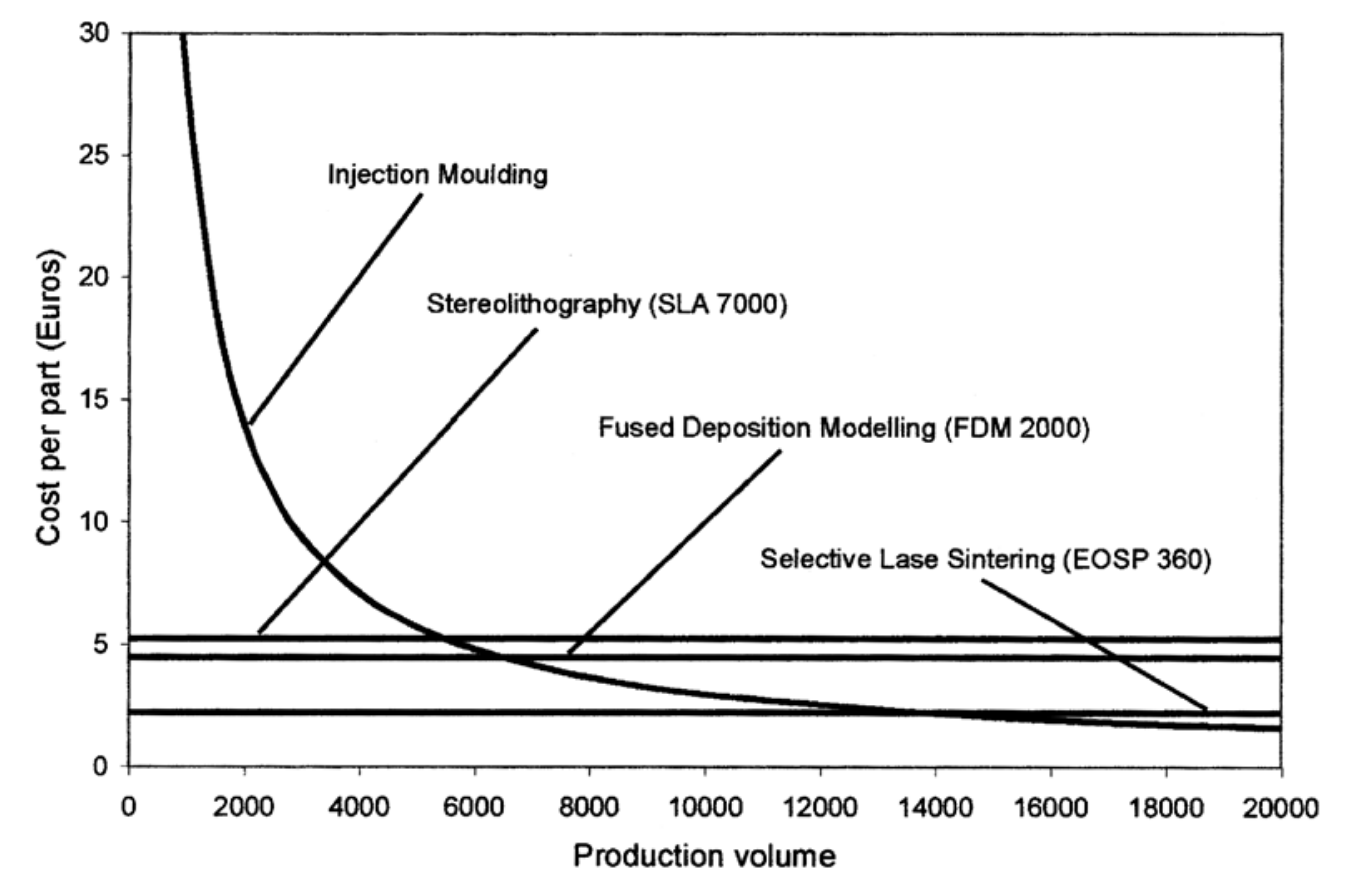
\includegraphics[width=0.55 \textwidth]{Images/costs.png}
    \caption[Traditional processes vs AM costs.]{Cost comparison for the manufacturing of a small plastic lever using different processes \cite{hopkinson_analysis_2003}.}
    \label{fig:costs}
\end{figure}
Furthermore, the initial machinery expenses were the primary cost factor in AM technologies. The authors believe these costs will decrease with mass adoption and technological advancements, thus reducing overall production costs. The real turning point for widely spread 3D printing occurred in the early 2010s, when patents for some polymers used in fused deposition modeling systems (FDM) expired. There was an absolute explosion of FDM 3D printer producers. We will discuss FDM shortly. Nowadays, additive manufacturing is employed in the production of small batches of finished products, sometimes even single-unit batches of highly customized products, or also in the prototyping phase.
These manufacturing processes do not intend to replace the traditional ones but rather allow us to expand the limits of what we can build. It is important to understand that additive manufacturing allows us to obtain components with mechanical functionalities and complexity unimaginable with traditional manufacturing processes but cannot be the only approach to production (at least for now).

%%%%%
%%%%%

% Additive Manufacturing Process Categories >>>
\section{Additive Manufacturing Process Categories} 
\label{sec:AMproc}
According to ISO/ASTM 52900 \cite{organization_isoastm_2015} and \citeauthor{gibson_additive_2015} (2015) there are seven different types of AM technologies: 
\begin{itemize}
    \item \textbf{Vat photo-polymerization processes} (VP). VP processes use radiation-curable resins or photopolymers that can be solidified using controlled light sources, usually ultraviolet radiation. Typically, it involves galvanometers to direct a laser beam or multiple directional light sources, such as controlled LEDs. The polymers used in this printing technology are usually acrylate-based or epoxy resins and industrial ceramic materials, such as alumina, zirconia, and silicon nitride. In recent years, new materials have been developed for the production of investment casting patterns \cite{3d_systems_investment_2023}, but also high technical performance material such as Cyanate Ester, which is used with Carbon Digital Light Synthesis\textsuperscript{TM} to produce pump turbines capable of withstanding high pressures (up to \numrange[range-phrase = --]{3800}{4000}\unit{\mega\pascal}) \cite{carbon_3d_carbon_2023}. The major advantages of this technology are the high level of accuracy of the finished products (up to \SI{0.05}{\milli\metre}), relatively high speed of manufacturing, and the variety of print sizes (ranging from tiny printers to larger ones, up to \qtyproduct{1000 x 800 x 500}{\milli\metre}. The disadvantages are that the finished prints require significant post-processing and that printers and the manufacturing process are still quite expensive. Moreover, material choices are limited to photopolymers only.
    \item \textbf{Fused filament fabrication} (FFF). FFF systems selectively extrude material as a filament through a heated nozzle. These processes are also called fused deposition modeling (FDM). These printers have a nozzle that is free to move in the horizontal plane and a system that moves it up and down along the z-axis (usually a threaded tube), allowing layer-wise material deposition. Typically employed materials are waxes, polyamide, acrylonitrile-butadiene-styrene, polyphenyl sulfone, polycarbonate, ceramics, and biocompatible or biodegradable materials. The main advantages of FFF systems include their widespread popularity and economic accessibility, as well as the variety of materials that can be used, such as ABS, which provides excellent structural properties, or PLA (polylactic acid), which can be extruded at relatively low temperatures and it is compostable. The drawbacks of this technology include lower print speeds and a lower achievable minimum resolution compared to other processes. We usually need to do some post-processing operations to achieve a satisfactory finishing.
    \item \textbf{Material jetting systems} (MJ). MJ is a technique that allows 3D printing of a piece using tiny droplets of liquid material selectively deposited onto a plate. Material jetting can be seen as the natural evolution of standard 2D inkjet printers but in three dimensions. MJ printers can use "cartridges" of materials and colors like traditional inkjet printers. One of the main advantages of MJ is the possibility of printing high-resolution multi-colored or multi-material objects. Initially, the materials used with this technology were waxes. Still, in recent years, the focus has been more on the deposition of acrylate photopolymers, in which droplets of materials are solidified with a UV lamp directly attached to the printing nozzle. The main advantages of MJ are the reduced material waste, as the deposition process is extremely precise (droplets of \numrange{25}{120} \unit{\micro\meter} at a rate of \numrange{0}{2000} \unit{drops / \second}), and the possibility of using different materials and colors simultaneously. The disadvantages of this solution are mostly the limited number of usable materials since only polymers and waxes or materials that are not excessively dense can be employed. Furthermore, the equipment required is relatively cheap, and the process can reach a remarkable printing speed.
    \item \textbf{Binder jetting systems}. Binder jetting is very similar to MJ. In binder jetting, a liquid binding agent called "binder" is selectively deposited in tiny droplets to solidify material powder, allowing different layers of powder to stick together. Due to the production method, the final objects may only sometimes be suitable for withstanding significant structural stresses and often require a long post-processing phase, which could increase variable costs. Binder jetting can be used with thermo-plastic polymers, metals, and ceramic materials. Compared to MJ, the significant advantages of this technology are the ability to use a much more vast range of materials and the higher printing speed. Moreover, it is possible to mix different powders to obtain final objects with specific mechanical features. However, printed parts often require a lot of post-processing work to improve the mechanical features and the finishing of the pieces.
    \item \textbf{Laminated object manufacturing} (LOM). In sheet lamination or laminated object manufacturing (LOM), layers of material are bonded together to form the final object. There are two possible approaches: "bond-then-form" and "form-then-bond." In the first case, the laminate is positioned and bonded to the substrate and then cut following the model contour. In the second case, the laminate material is cut, placed on the substrate, and bonded to the underlying layer. LOM techniques allow the usage of wood, thermo-plastic polymers, industrial ceramics, paper, polyvinyl chloride, and composite materials. The significant advantages of LOM are the ability to print large parts quickly and the lower equipment fixed costs compared to other types of AM processes.
    \item \textbf{Powder bed fusion} (PBF):  In these additive manufacturing techniques, a concentrated energy source is used to melt layers of powder selectively. Usually, the energy source is a laser (Selective Laser Sintering or SLS) or an electron beam (Electron Beam Melting or EBM), and the materials used can be polyamides, nylons, elastomers, and metals such as stainless steel, titanium, aluminum, cobalt, and copper. This AM technique is widely used for direct manufacturing and allows for producing finished objects with excellent mechanical properties and surface finishes.
    \item \textbf{Direct energy deposition} (DED): In DED, a concentrated heat energy source is used to melt material as soon as it is deposited selectively. Depending on the energy source used, we can further divide the processes into laser, electron beam, and plasma metal deposition. Moreover, depending on the shape of the material used, we can distinguish between powder-fed and wire-fed systems. Finally, depending on the direction in which the material is fed, we can distinguish between off-axis feeding, in which a side-mounted incident nozzle deposits the material, and coaxial feeding systems, in which the powder or wire material is deposited co-axially with the energy beam. The main advantage of DED is that it can be used to add parts to existing components or for repairs with a minimum need for support structures. There are several powders and printing area sizes available. However, DED has a lower accuracy compared to PBF, which makes DED unsuitable for producing complex shapes.
    \end{itemize}

% <<< End of Additive Manufacturing Process Categories

%%%%%
%%%%%

\section{Aim and Structure of the Work}
\label{sec:aimwork}
\begin{figure}
    \centering
    \subfloat[\label{fig:bugatti}]{
        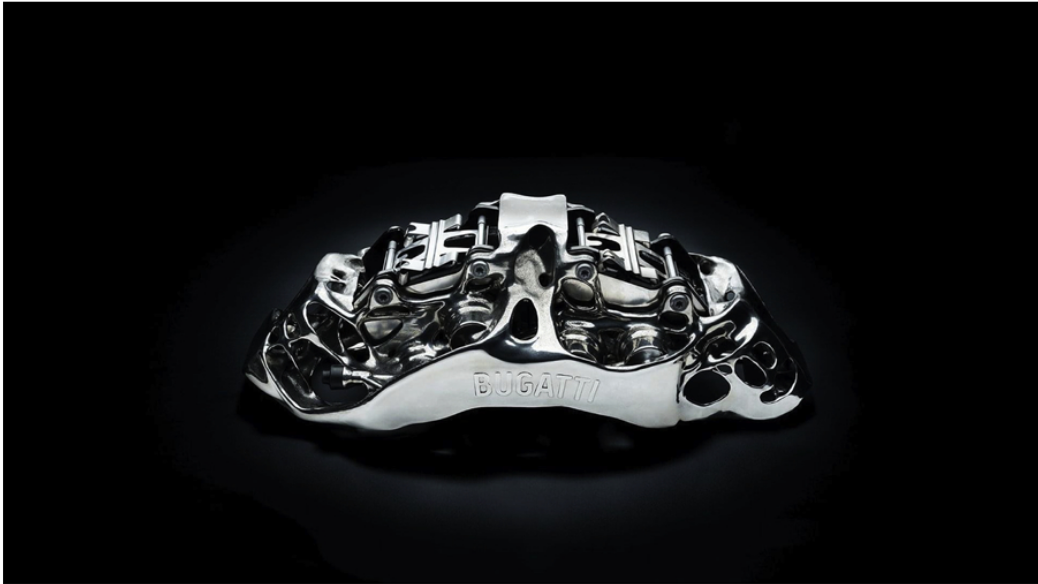
\includegraphics[scale=0.4]{Images/bugatti.png}
    }
    \quad
    \subfloat[\label{fig:supporto}]{
        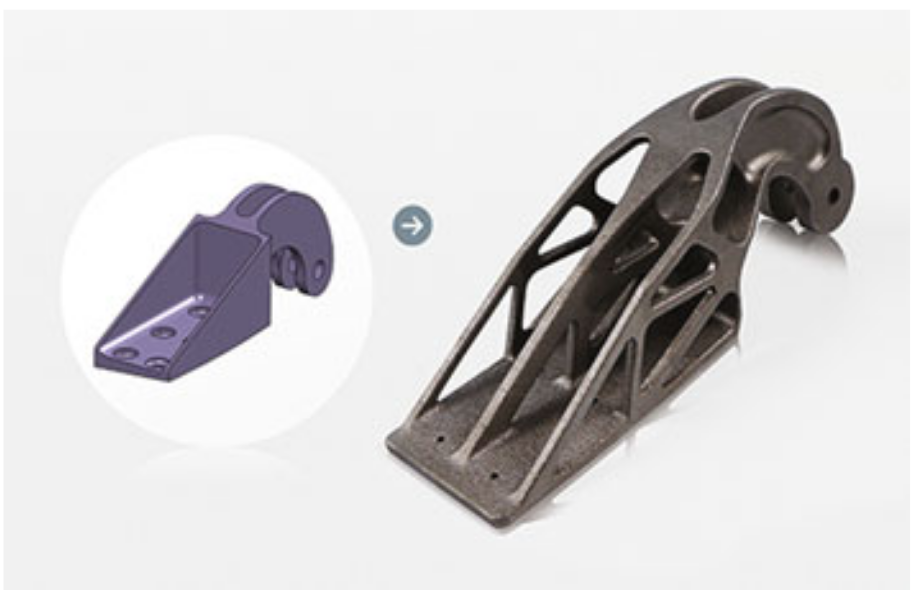
\includegraphics[scale=0.4]{Images/supporto.png}
    }
    \caption[Functional AM part printed in metal.]{On the left, a Bugatti brake caliper, one of the world’s largest functional parts produced in titanium alloy Ti6Al4V by AM. On the right, we can see support used in the aerospace industry. From \citeauthor{du_plessis_beautiful_2019}.}
    \label{fig:funcpart}
\end{figure}
In recent years, additive manufacturing processes for metallic parts, especially the so-called powder bed fusion processes, have revolutionized various industries, including aerospace, automotive, and energy. PBF processes are currently the most promising AM technology for printing structurally sound and functional components. Indeed, these processes are also used to create components that play a critical role during their use, often for safety reasons. Consider, for instance, the importance of the brake system shown in Fig. \ref{fig:bugatti}. Imagine the repercussions if the braking system failed on a Chiron that is speeding at \SI{350}{\kilo\metre /\hour}, or if aerospace support, like the one in Fig. \ref{fig:supporto}, may break, causing a \SI{8500}{\metre} fall of a heavy piece. For these reasons, as shown in Fig. \ref{fig:vchain}, the AM chain is particularly articulated, mainly due to the importance of the testing and certification phases. Data collected from process monitoring in AM presents a unique opportunity (compared to traditional manufacturing) for early defect detection or new non-destructive testing techniques.
\begin{figure}
    \centering
    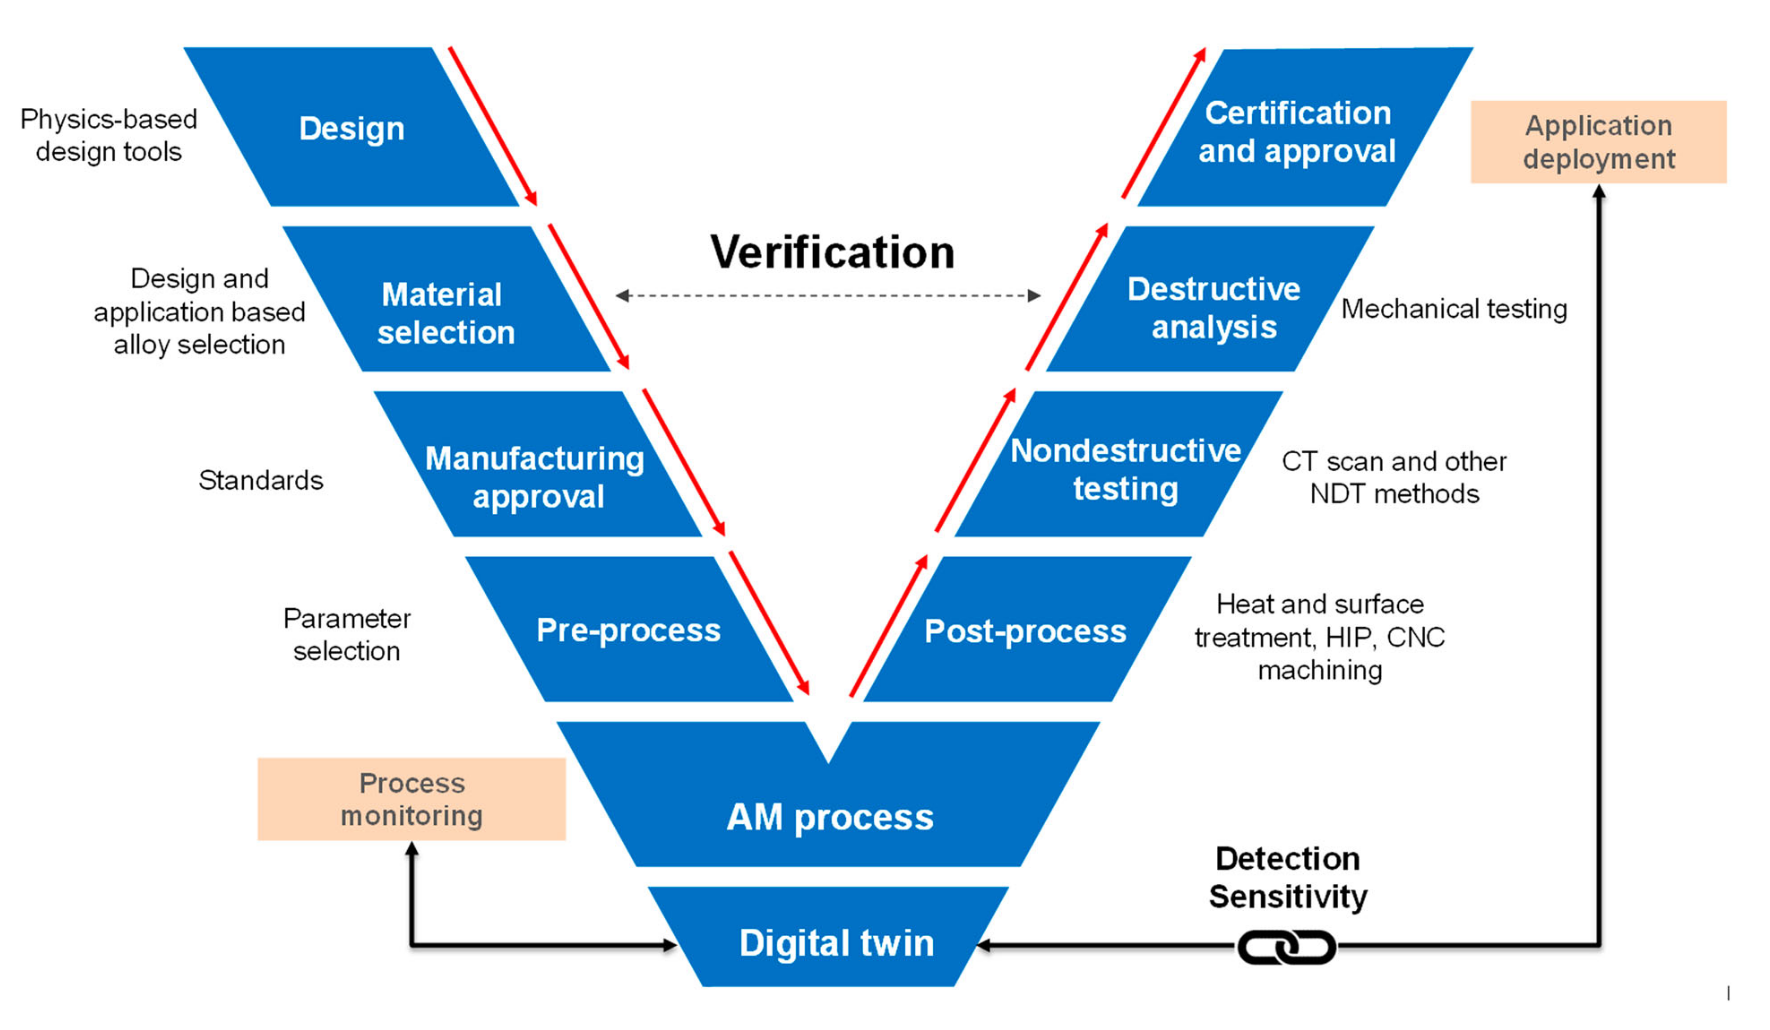
\includegraphics[width=0.65 \textwidth]{Images/v.png}
    \caption[AM process chain.]{V-shaped process chain for AM from design to certification \cite{moshiri_performance_2023}.}
    \label{fig:vchain}
\end{figure}
Quality control, defect detection, and ensuring the production process adheres to standards are crucial now more than ever. The temperature, particularly in additive manufacturing for metallic parts, significantly influences the mechanical properties of the finished product, as demonstrated in \citeauthor{williams_situ_2019} (2019). Indeed, the temperatures reach much higher peaks, and the cooling process is more dynamically complex. Anyone who has experience with "classical" FDM 3D printing for PLA would notice that the filament cools down in seconds. On the other hand, with metallic PBF printing, one must wait considerably longer before the final piece is extracted from the production chamber. Moreover, many additional factors could affect the temperature reached by the material during the PBF printing process and the consequent cooling process. This thesis aims to present a state-of-the-art review of identifying the so-called hot spots in PBF processes using machine learning algorithms. Hot spots are localized areas characterized by elevated temperatures for a sustained time and slower cooling drift, often attributable to their proximity to adjacent loose powder. The overheating leads to defects in the finished product.

This thesis is structured as follows. Chapter~\ref{ch:Metal_AM}, I will comprehensively describes PBF processes for 3D printing of metal parts, the necessary technologies, materials, and some potential applications. Chapter~\ref{ch:defects} outlines the most common defects in PBF processes, with a particular emphasis on the aforementioned hot spots, their causes, and the different monitoring systems used in AM. Chapter~\ref{ch:state_ot_the_art} is a literature review to present the state-of-the-art in hot spots detection using machine learning algorithms. The methods for the systematic review is explained in Appendix~\ref{ap:research}. Chapter~\ref{ch:baggingvoronoi} presents the bagging voronoi classification algorithm as an innovative approach that might lead to a deeper understanding of the hot spots phenomenon leveraging functional data, as well as providing a powerful non-destructive analysis tool for thermal profiles. Chapter~\ref{ch:conclusions} conclude the thesis and propose some research streams that could be explored further. Finally, Appendix~\ref{ap:Python}, proposes a simple Python \cite{python_software_foundation_python_2023} implementation of the algorithm proposed in Chapter~\ref{ch:baggingvoronoi}.
% ---------


% Introduction ---------
\chapter{Powder Bed Fusion Processes and Lattice Structures}
\label{ch:Metal_AM_and_lattice}%
\setlength{\tabcolsep}{10pt}
In this section, we will focus on additive manufacturing for metal lattice structures using a PBF process. In section \ref{sec:pbf_proc}, we will discuss how 3d printers for PBF process with metal materials, while in section \ref{sec:lattice}, we will delve into lattice structures.
\section{Powder Bed Fusion Processes}\label{sec:pbf_proc}
As we have already discussed in section \ref{sec:AMproc}, powder bed fusion processes can be further divided into laser powder bed fusion also called selective laser sintering (SLS) or electron beam powder bed fusion also called electron beam melting (EBM). Despite the fact that the two technologies are based on two different ideas and some differences in components between 3D printers, the two processes share several common elements and points. Since the thesis concerns lattice structures printed in metal, in this section we will delve into PBF technologies suitable for metallic materials. 
\begin{figure}[H]
    \centering
    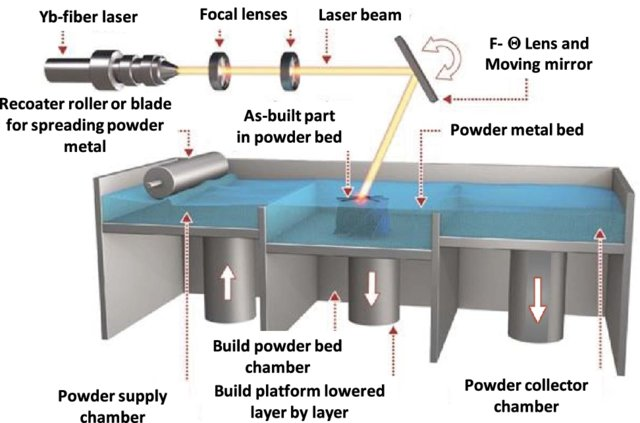
\includegraphics[scale=1.3]{Images/PBF.jpg}
    \caption[Laser PBF in AM.]{Laser powder bed fusion process in additive manufacturing. Adapted from \cite{ozel_focus_2020}.}
    \label{fig:PBF}
\end{figure}

All PBF 3D printers consist of two basic components: the powder bed, which is a movable container along the z-axis for the metallic powder, and a highly concentrated energy source. 
Firstly, the plate mounting is calibrated and a vacuum is created inside the printer's process chamber or a regular flow of inert gas is introduced to obtain controlled and uniform melting. In the industrial context, directing an inert gas is preferred to maintaining a vacuum throughout the printing process. This is because it's difficult to maintaining a vacuum throughout the printing process and lowering the pressure in the process chamber can lower the boiling point of the metals, leading to the formation of an excessive amount of vapor, which can affect the effectiveness of the laser. Once the vacuum or inert gas flow is established, the roller or blade responsible for distributing the powder performs a rapid powder recoating and an electric resistance located under the powder bed preheats the powder at a temperature of \SI{500}{\degreeCelsius}. This operation help to reduce the gap between the temperature of the chamber and the metal's melting temperature. However, the preheating operation is not always necessary, and in the case of EBM, it is not even required. We will discuss the reason why later. after which the printing can begin. After these preliminary operations, the printing process can begin. A scanning system composed of a laser diode and a galvanometric mirror system selectively melts the metal layer by layer, alternating with the powder distribution tool on the print bed, layer after layer. LASER is an acronym that stands for "Light Amplification by Stimulated Emission of Radiation," and it is a monochromatic beam of photons characterized by low divergence and a focal spot size of \SIrange[range-phrase = --]{30}{80}{\micro\metre}.
\begin{figure}[H]
    \centering
    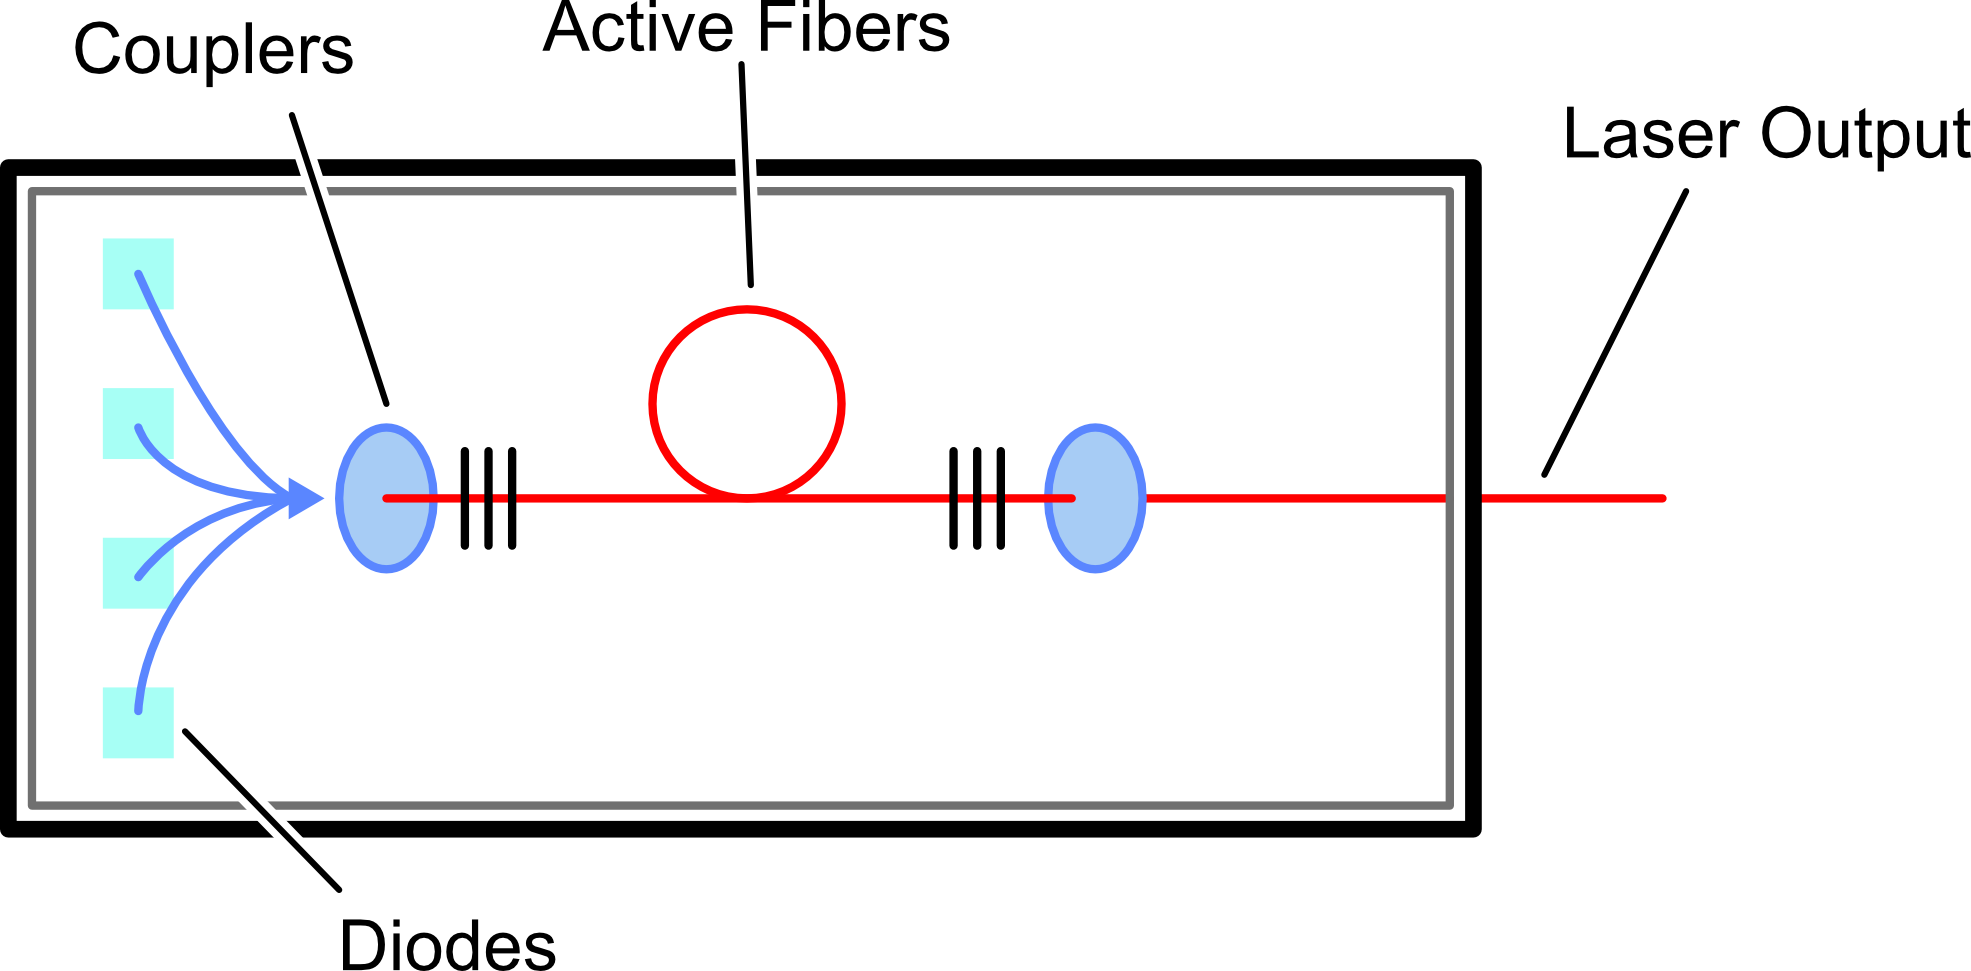
\includegraphics[scale=0.5]{Images/laser2.png}
    \caption[Laser schema.]{Active fiber laser schema.}
    \label{fig:laser}
\end{figure}
Laser equipment has the capability to generate powers in the range of thousands of watts and can focus to beam spot sizes of fractions of a millimeter. These small spot sizes have the potential to create minuscule molten pools that can melt at extremely high travel speeds, reaching up to several meters per second. Nowadays, almost all lasers used in AM rely on active optical fiber sources, fig. \ref{fig:laser}. In this laser technology, optical pump diodes are coupled to an active laser fiber that has a unique reflective coating and Bragg gratings. These components enable the laser light to reflect back-and-forth along the length of the fiber, producing a coherent beam of light at the output of the laser. Additional optical fibers are commonly used to deliver and contain the light energy, providing a robust, flexible, and fully enclosed beam path for beam delivery \cite{milewski_additive_2017}. The energy transferred from the laser to the powder bed depends on the laser power (\SIrange[range-phrase = --]{100}{1000}{\watt}, the light-absorbing capacity of the material, and the scanning speed, which can be controlled by modifying the angular velocity of the galvanometer.

\begin{figure}[H]
    \centering
    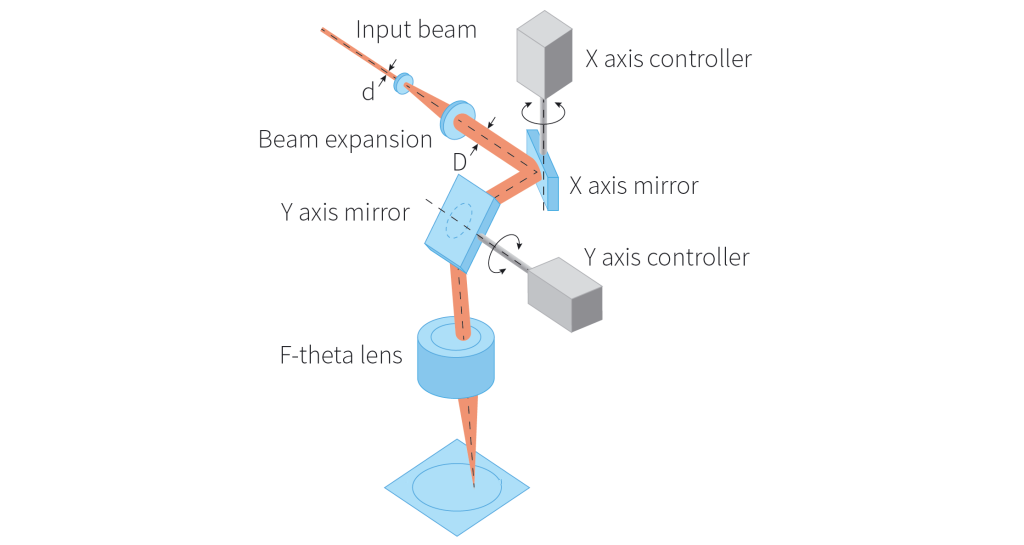
\includegraphics[scale=0.5]{Images/galvanometro.png}
    \caption[Galvanometric system.]{Dual-axis galvanometric system.}
    \label{fig:galvano}
\end{figure}
The galvanometric system, fig. \ref{fig:galvano}, system consists primarily of two mirrors rotating along their axis, enabling the laser beam to be directed, and a series of f-theta lenses that facilitate rapid laser movement and precise focusing of laser beam. After completing the printing process, it is necessary to allow the object to cool down. Although supports are not always necessary in PBF processes as the powder gives support to the object itself, they may need to be inserted to ensure uniform heat transmission during both the printing and cooling processes. Once the object has cooled down, any excess powder can be removed. The excess powder can be recycled and reused after undergoing some preliminary processing and conformity controls. Finally, if required, post-processing operations can be carried out, such as removing any supports, surface finishing, and annealing. This is especially important if the cooling process inside the chamber has created an undesired microstructure in the final cooling part.\\
In EBM printers, the process is fundamentally the same as in laser printers, with metal powder selectively fused from a tray. However, there are several significant differences. Firstly, the energy source is not a laser (i.e., a beam of photons) but rather an electron beam. Secondly, the preheating stage is not accomplished through the use of an electric resistor, but instead through the use of the electron beam itself. But how does an electron beam function? To produce an electron beam, an electric current is passed through a tungsten filament. The resulting electron beam is then directed through a Wehnelt cylinder, which, when negatively or positively charged, respectively blocks or allows the passage of electrons.

\begin{figure}[H]
    \centering
    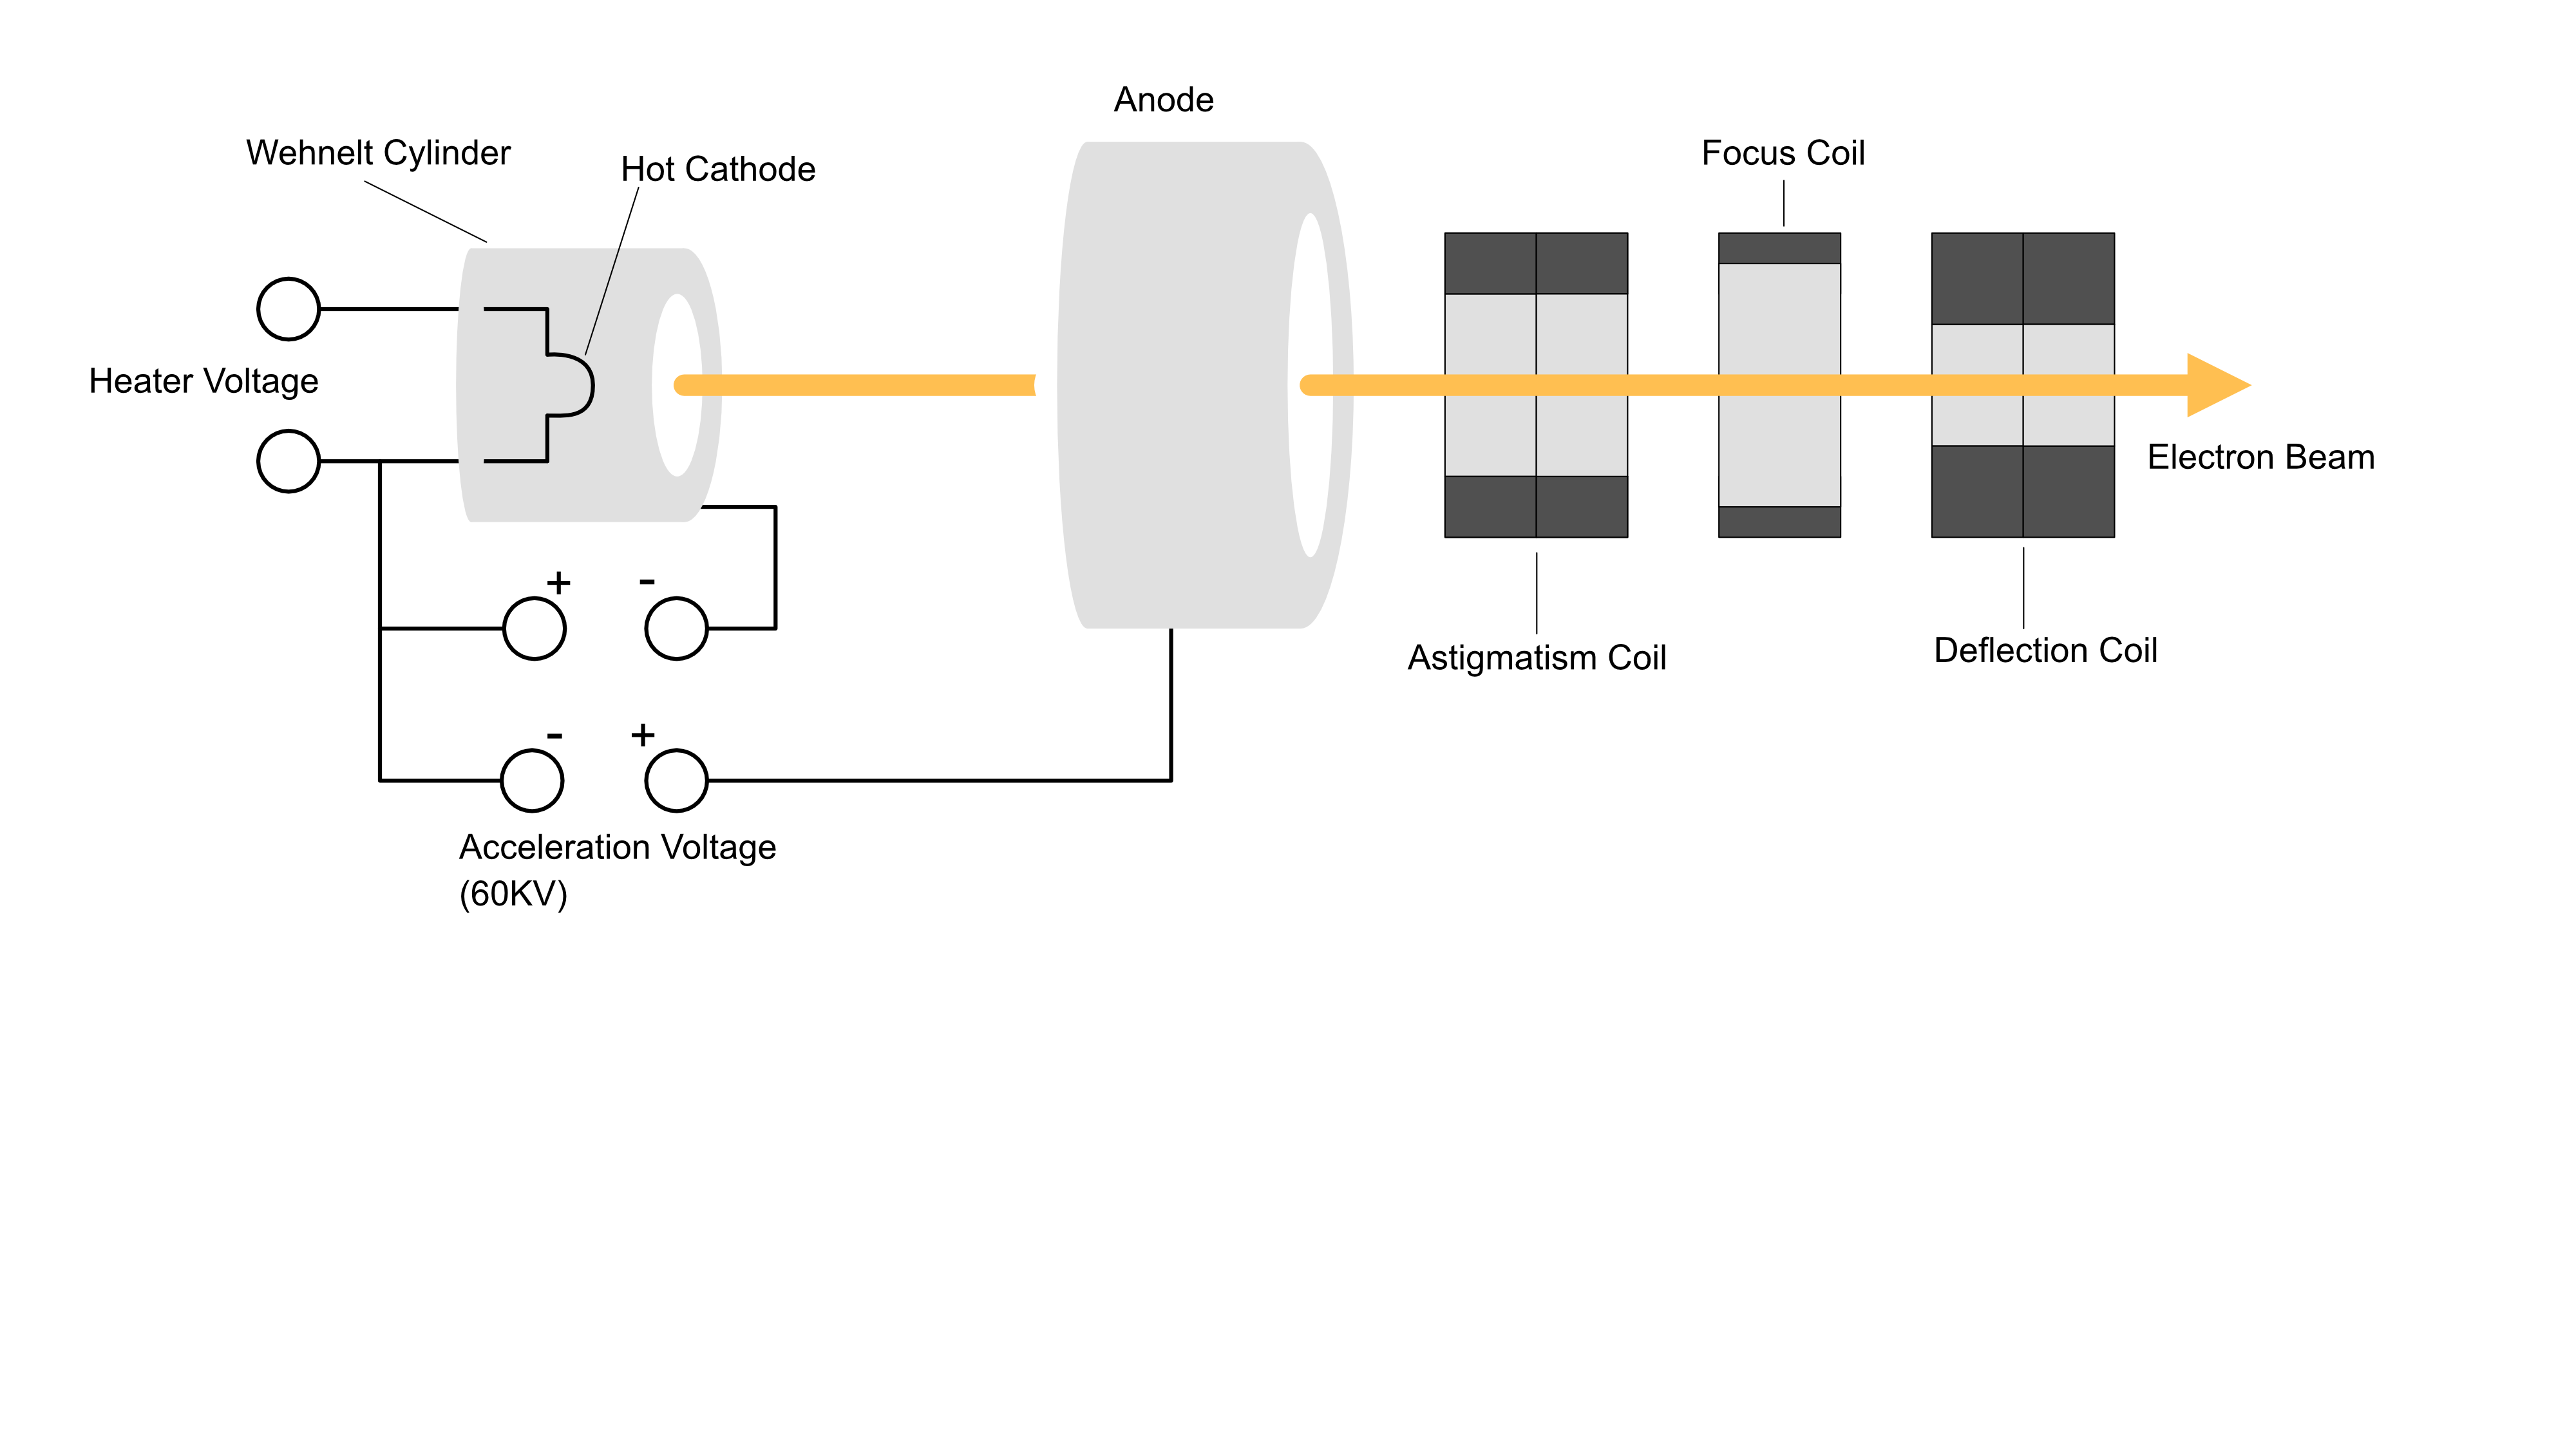
\includegraphics[scale=0.5]{Images/EBM.png}
    \caption[Electron gun schema.]{Electron gun schema.}
    \label{fig:electrongun}
\end{figure}

A diagram of the electron gun beam's structure can be seen in fig. \ref{fig:electrongun}. Finally, the electron beam passes through an anode charged with a voltage of up to \SI{60}{\kilo\volt}, which accelerates the electrons and allows the beam to be directed into the column through magnetic lenses. Unlike SLS printers that use optical lenses, the lenses in EBM printers are magnetic and use a magnetic field to alter the path of the electron beam. As the beam passes through these lenses, the astigmatic lenses adjust the shape of the electron beam spot, the focus coil changes the spot size, and the deflection coil moves the beam along the x and y axes. Like SLS printers, the EBM printer requires a vacuum inside the printing chamber, and a minute amount of helium must be continuously injected into the chamber to prevent the accumulation of electric charges due to any residual electrons on the powder bed. To put the minuscule amount of helium required into perspective, consider that the starting pressure is \SI{0,05}{\pascal}, and the pressure with helium flow is bout \SI{0,2}{\pascal} (atmospheric pressure is \SI{1,01325e5}{\pascal}). The second major difference, as mentioned earlier, is that the preheating phase does not occur through an electric resistance but rather through an initial scan of the electron beam at two distinct moments. During the first phase, the entire powder bed is scanned, and during the second phase, only the subregions of the powder bed that will actually be printed are scanned. These preheating phases are useful in avoiding the so-called "smoke effect," an effect caused mainly by the vacuum atmosphere inside the print chamber and electrostatic repulsion in the powder. Furthermore, the preheating phase is necessary for obtaining final objects with better performance and reduces the need for support structures during printing. This allows for the use of the entire volume of the powder bed container when printing, and even printing multiple objects on top of each other, since there would be no printing supports interfering with them. This dual pre-heating phase causes the excess powder to solidify around the printed piece and need to be removed with compressed air mixed with the same loose powder used during printing process in order to obtain a slight smoothing effect. Moreover, printing chamber must be shielded against X-rays because when the electron beam hits the metal powder, some electrons are emitted from the metal's atom inner orbital, leading to the formation of the aforementioned rays. Another structural difference of an EBM printer can bee seen in fig.~\ref{fig:ebm_printer}. Due to the vacuum inside the print chamber and the consequent lowering of the metal's vaporization temperature, a heat shield is required around the chamber to prevent the vaporized metal from condensing and creating a film on the entire printer structure. Essentially, the heat shield acts as a physical barrier that allows for easy removal and disposal of the metal film created during the printing process.
\begin{figure}[H]
    \centering
    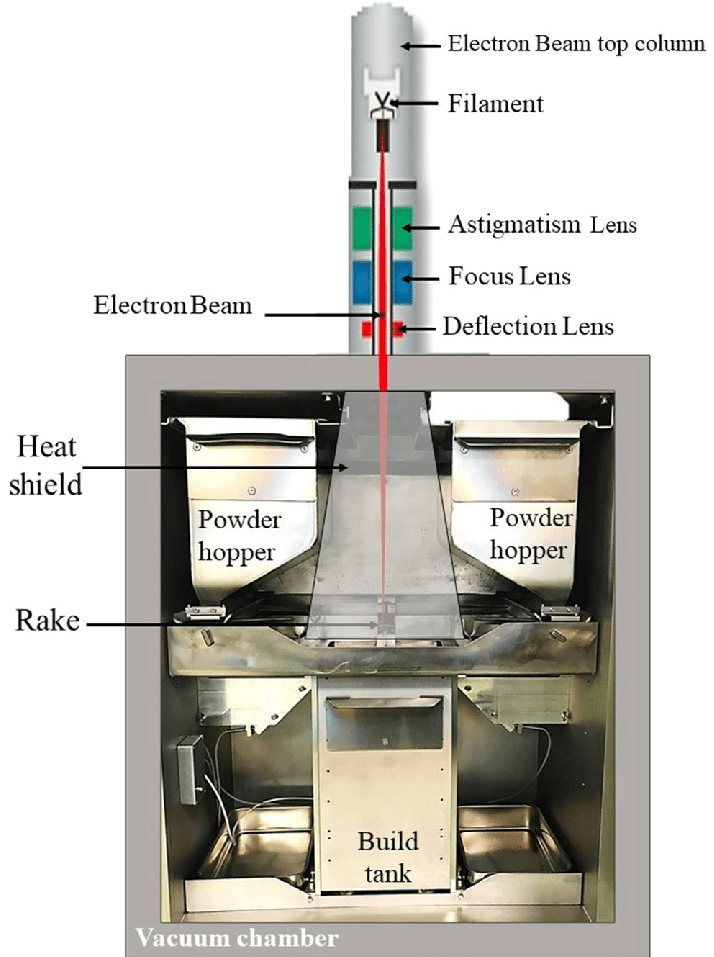
\includegraphics[scale=0.3]{Images/A-schematic-of-electron-beam-melting-EBM.png}
    \caption[EBM 3d-printer.]{Electron beam melting 3d-printer, from        \citeauthor{azam_-depth_2018} (\citeyear{azam_-depth_2018}).}
    \label{fig:ebm_printer}
\end{figure}
 There are also differences in the materials used for printing. In EBM printing, usually metal powder size is slightly larger than the powder used in laser printing, with a particle size of approximately \SIrange[range-phrase = --]{40}{105}{\micro\meter} against the \SIrange[range-phrase = --]{15}{45}{\micro\meter} in SLS processes. This is needed in order to prevent excessive "smoke effect". Furthermore, metal powder must be made of metals that exhibit good electrical conductivity. Indeed, in EBM also highly reflective metals can be used, because unlike photons, electrons are not repelled by mirrored surfaces since they penetrate the material thanks to the material's own electrical conductivity.
\subsection{Metal Powders Sintering}
%%%%%%
%%%%%%
\section{Metal Powders for AM} \label{sec:metalpowders}
As we have seen in the section \ref{sec:pbf_proc}, PBF processes require metal powder for the process. Various metallic materials can be transformed into powders suitable for use in additive manufacturing processes, and can be applied in different sectors according to their mechanical properties. The table \ref{table:materialAMmetal} presents some examples of metallic materials that can be used for this purpose. 

\begin{table}[H]
\centering 
    \begin{tabular}{|l l l|}
    \hline
%    \rowcolor{bluepoli!40}
     \textbf{Material} & \textbf{Examples} & \textbf{Applications}\\
    \hline \hline
    \textbf{Stainless steel} & 316L, 174-PH, MS1, M300 & Food, biomedical, consumer \T\B\\
    \hline
    \textbf{Ni-alloys} & In625, In718, In939 & Energy, motorsport\T\B\\
    \hline
    
    \textbf{Al-alloys} & AlSi12, AlSi10Mg & Lightweight, aerospace, aviation\T\B\\
    \hline

    \textbf{CoCr-alloys} & CoCrMo & Dental, biomedical\T\B\\
    \hline

    \textbf{Ti-alloys} & Ti6Al4V, CP Ti & Biomedical, lightweight, aerospace\T\B\\
    \hline

    \textbf{Tool steel} & Maraging 18Ni300 & Tooling, aerospace, automotive\T\B\\
    \hline

    \textbf{Cu-alloys} & Bronze & Energy, heat exchanger\T\B\\
    \hline

    \textbf{Precious} & Au, Pt, Ag & Jewellery, design\T\B\\
    \hline
    
    \end{tabular}
    \\[10pt]
    \caption{Material availability for metal AM.}
    \label{table:materialAMmetal}
\end{table}




In the vast majority of cases, these powders are produced using atomization processes that exploit various physical methods to generate micro-particles characterized by a spherical shape and of which chemical purity depends on the method used. The inefficiency and cost of atomization processes used for manufacturing metal powders is the reason why, in the case of specific high-quality powders, the powder price can be up to 10 times the price of raw metal. It has been demonstrated that powders made of irregular microparticles with low chemical purity can lead to structural defects in the final parts, resulting in lower performance \cite{deng_origin_2020}. Therefore, over the years, increasingly complex and expensive processes have been developed to obtain higher-quality powders. In figure \ref{fig:atom} there are various atomization processes schematically depicted.
\begin{figure}[H]
    \centering
    \subfloat[Water atomization process.\label{fig:wateratom}]{
        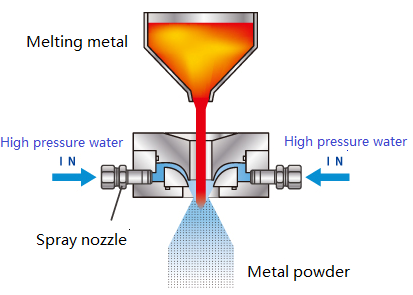
\includegraphics[scale=0.6]{Images/wateratom.png}
    }
    \qquad
    \subfloat[Gas atomization process.\label{fig:gasatom}]{
        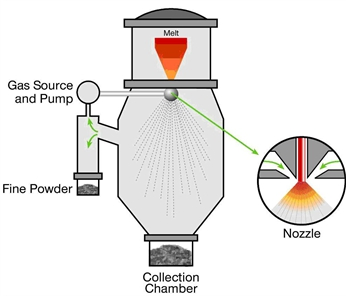
\includegraphics[scale=0.6]{Images/gasatom.png}
    }
    \qquad
     \subfloat[Plasma atomization process.\label{fig:plasmaatom}]{
        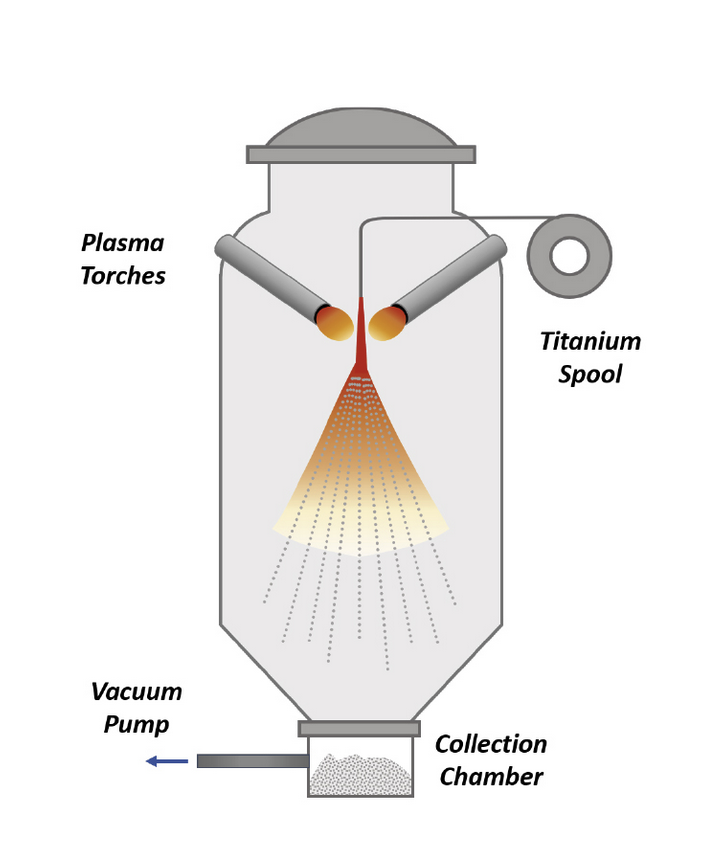
\includegraphics[scale=0.4]{Images/plasma.png}
    }
    \qquad
    \subfloat[Rotating electrode process.\label{fig:repatom}]{
        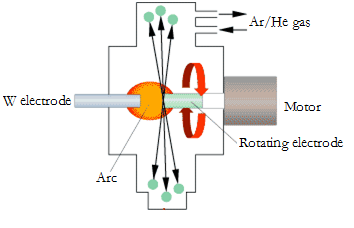
\includegraphics[scale=0.7]{Images/repatom.png}
    }
    
    \caption[Atomization processes]{Different atomization processes. Pictures from \cite{material_technology_innovations_co_rotating_nodate, material_technology_innovations_co_water_nodate, material_technology_innovations_co_gas_nodate, inovar_communications_ltd_metal_2020}.}
    \label{fig:atom}
\end{figure}
The process of \emph{water atomization}, fig. \ref{fig:wateratom}, of metals involves the production of small droplets of molten metal by exposing a stream of the molten metal to a high-pressure jet of water. The water atomization process is typically carried out in a chamber where the molten metal is injected into a nozzle that directs the stream of liquid metal towards a high-pressure jet of water. As the molten metal comes into contact with the water, it rapidly cools and solidifies, forming small droplets that are collected at the bottom of the chamber. The size and shape of the metal droplets produced during the water atomization process can be controlled by adjusting various parameters such as the temperature of the molten metal, the pressure of the water jet, and the distance between the nozzle and the water jet. By controlling these parameters, it is possible to produce metal powders with a range of particle sizes between \SIrange[range-phrase = --]{1}{500}{\micro\metre}. The output-to-input ratio for this process is approximately 95\%, which means that from \SI{1}{\kilo\gram} of raw metal, it is possible to obtain up to \SI{950}{\gram} of powder on average. Compared to other powder production methods, the water atomization process offers several advantages including high production rates, the wide range of particle sizes obtainable, high production rates, and the fact that metal ingots can be used as process input, which shortens the supply chain of this production process. On the other hand, the major disadvantages are the low chemical purity, irregular shape as can be seen in fig. \ref{fig:waterpow}, and the need for extensive post-processing to obtain a decent-quality product. Moreover, it cannot be used with reactive materials such as titanium and aluminum.

\emph{Gas atomization}, fig. \ref{fig:gasatom}, can be performed using a variety of gases, depending on the specific application and metal being processed. The most commonly used gases for gas atomization are inert gases such as nitrogen, argon, and helium, even if the latter is barely used in industrial applications due to its high cost. Inert gases are preferred because they do not react with the molten metal and do not introduce impurities into the metal powders. Metal ingots are molten and the flow is rapidly solidifying through exposure to a high-pressure stream of gas. Main advantages of this process are the high production rate, the wide range of obtainable particles, its applicability to reactive materials, and its ability to ensure good chemical purity. The main drawbacks, on the other hand, are mostly related to the porosity of the resulting powder and the formation of small satellite particles. Additionally, the cost of the process is higher if compared to water atomization.

The process of \emph{plasma atomization}, fig. \ref{fig:wateratom}, involves the usage of high-temperature plasma torches to melt metal wire. The high-energy plasma arc is created by passing an electric current through a non-consumable tungsten electrode and an inhert gas jet to direct the welding arc into a focused area. As the molten metal droplets are expelled from the plasma jet, they rapidly solidify, sometimes also thanks to the water-cooled chamebr, and break up into small, spherical powders, which are then collected in a container. The plasma atomization process offers several advantages over other powder production methods, including the ability to produce powders from reactive metals and the ability to produce extremily spherical shape. Plasma atomization can also produce powders with very high purity levels, as the high temperature of the plasma jet helps to eliminate impurities in the molten metal. However, plasma atomization is more expensive than other powder production methods due to the need for specialized equipment and the high energy consumption required to generate the plasma arc. The process can also be challenging to control, as variations in process parameters can affect the size, shape, and purity of the resulting metal powders. Lastly, powders produced using this method has a low size range of about \SIrange[range-phrase = --]{1}{200}{\micro\metre}. 

In \emph{rotating electrode process}, a consumable metal electrode is rotated at high speeds while it is melted by an electric arc. As the molten metal is exposed to the high-velocity inert gas stream, it rapidly solidifies and breaks up into small droplets, which are then collected at the bottom of the atomization chamber. Due to its high cost, this production method is typically used when it is necessary to obtain a metal powder with a perfectly spherical shape and without any impurities. If we take a look at fig. \ref{fig:reppow}, we can easily grasp the potential of this technology in obtaining perfect spherical micro-particles.
\begin{figure}[H]
    \centering
    \subfloat[\label{fig:waterpow}]{
        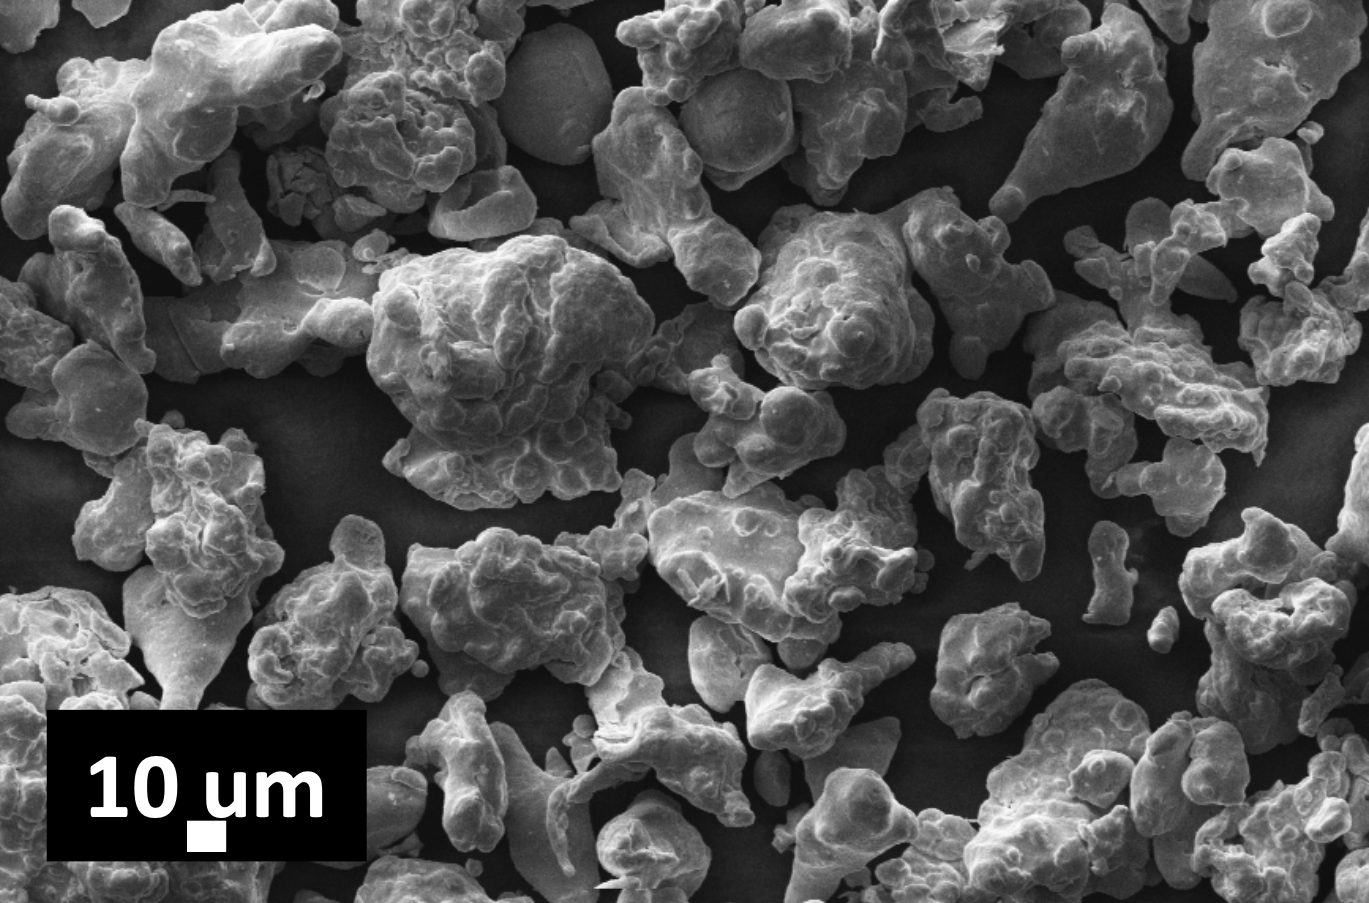
\includegraphics[scale=0.22]{Images/waterpow.png}
    }
    \qquad
    \subfloat[\label{fig:gaspow}]{
        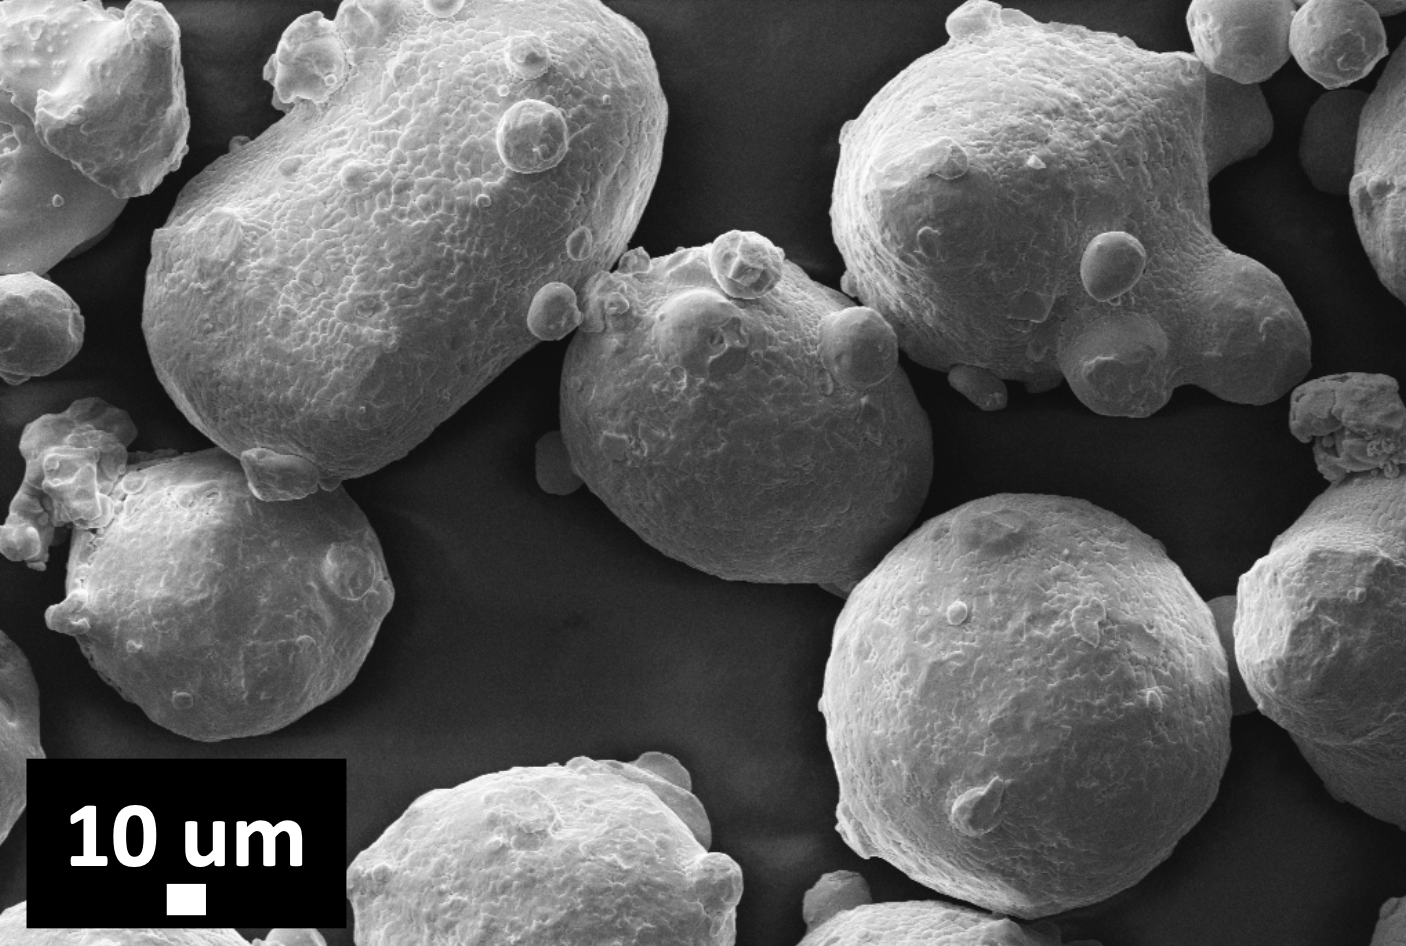
\includegraphics[scale=0.21]{Images/gaspowd.png}
    }
    \qquad
     \subfloat[\label{fig:plasmapow}]{
        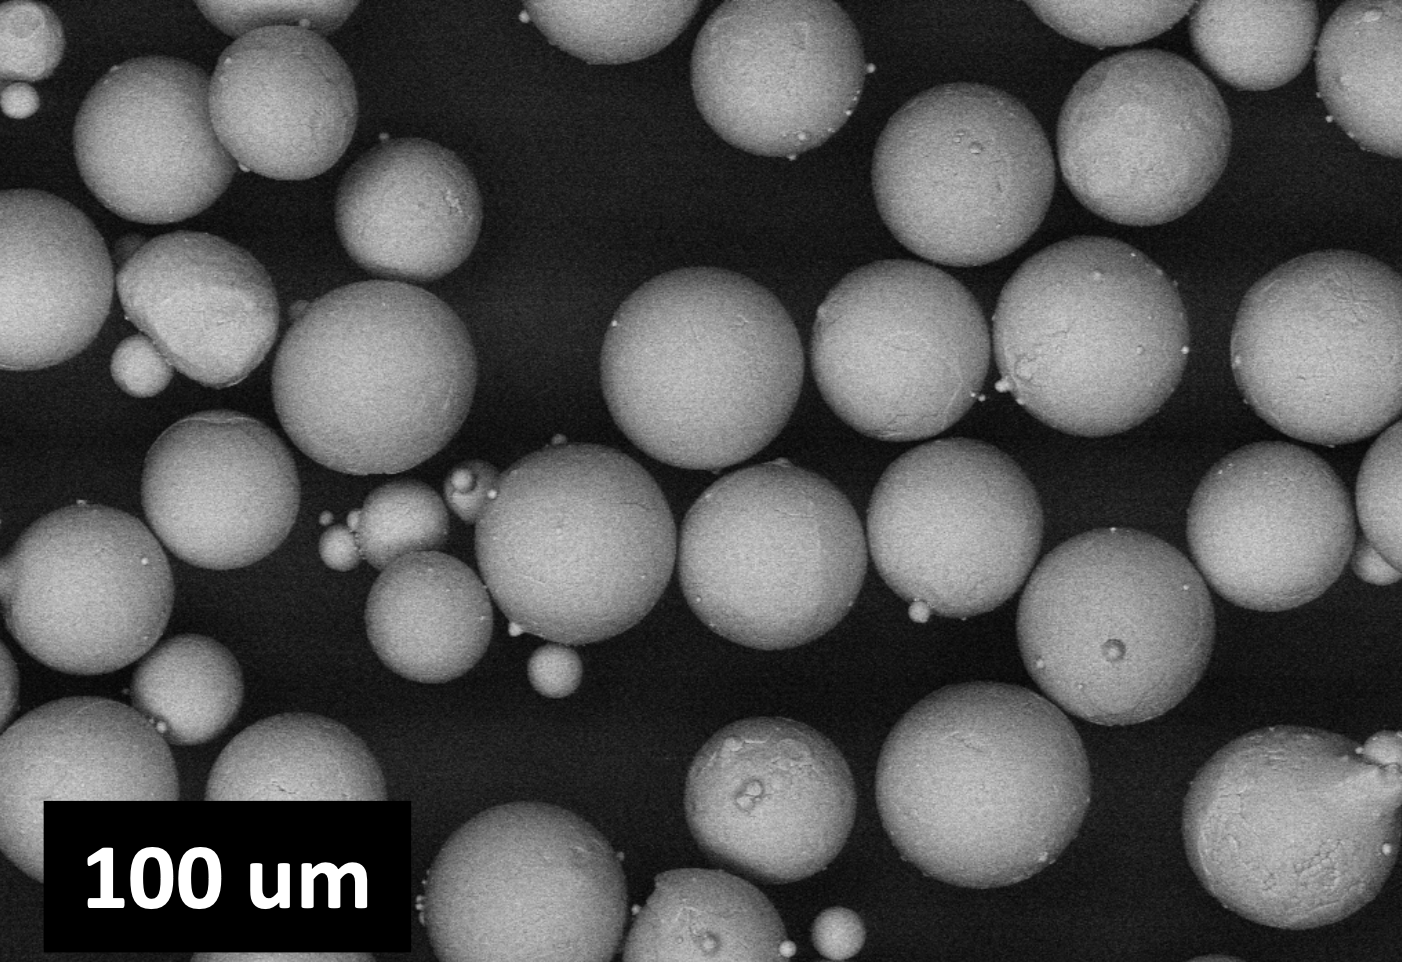
\includegraphics[scale=0.22]{Images/plasmapowder.png}
    }
    \qquad
    \subfloat[\label{fig:reppow}]{
        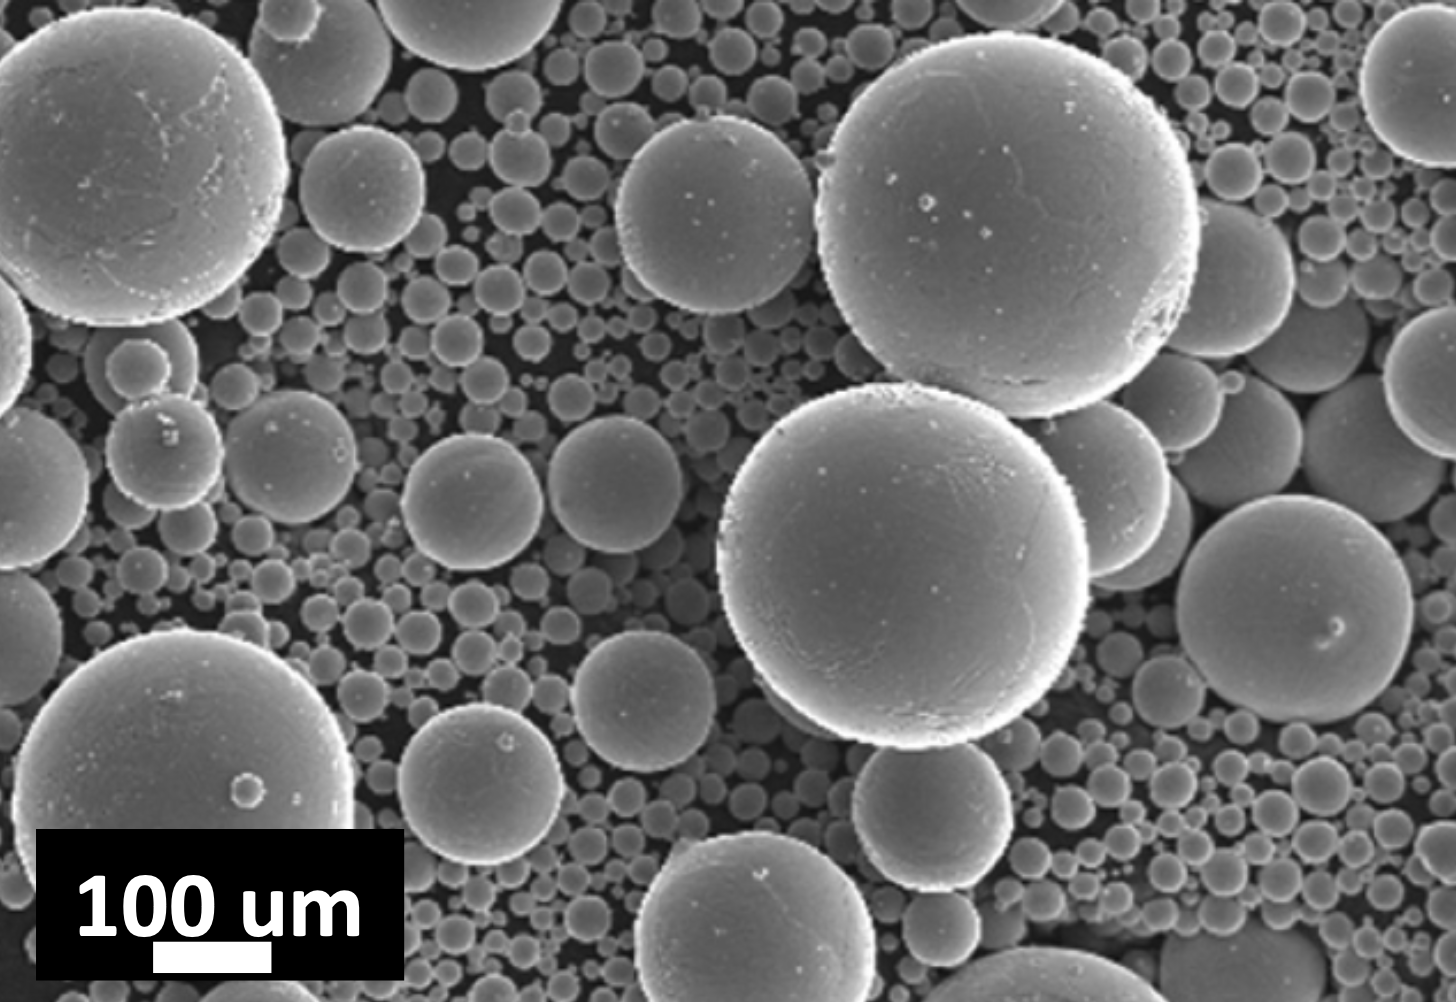
\includegraphics[scale=0.21]{Images/erppowder.png}
    }
    
    \caption[Powders from atomization processes]{Micro-particles obtained by water atomization (a), gas atomization (b), plasma atomization (c) and rotating electode process (d).}
    \label{fig:powders}
\end{figure}
%%%%%%
%%%%%%
\section{Lattice Structure and Cellular Material} \label{sec:lattice}
According to ISO/ASTM 52900 \cite{international_standard_organization_isoastm_2015}, lattice structure are "three dimensional geometric arrangement composed of connective links between vertices (points) creating a functional structure". So, lattice structures are three-dimensional structures made up of different connected single elements called "cells" that can have different shapes, designed to meet the needs of the final object. These objects are distinguished by empty spaces within the structure. These structures can only be obtained thanks to layer-wise additive manufacturing technologies, since they allow us to design and to manufacture objects with complex designs and intricated parts. In recent years, the biomimicry technique has also spread to additive manufacturing, and lattice structures are the natural manifestation of this technique. Biomimicry is a set of design techniques that allow us to take inspiration from nature to find solutions to engineering problems or to design functional components that can be used in engineering applications \cite{pathak_biomimicry_2019, du_plessis_beautiful_2019}. Nature, over the past 3.8 billions years, has been able to find the most efficient way to develop functional solutions to evolutionary problems characterized by immovable constraints, whether they are determined by the organism itself or by external factors. For example, think of the wings of dragonflies in fig. \ref{fig:dragonfly}, a lightweight, completely transparent structure that allows flight, allowing them to fly unnoticed by predators. 
\begin{figure}[H]
    \centering
    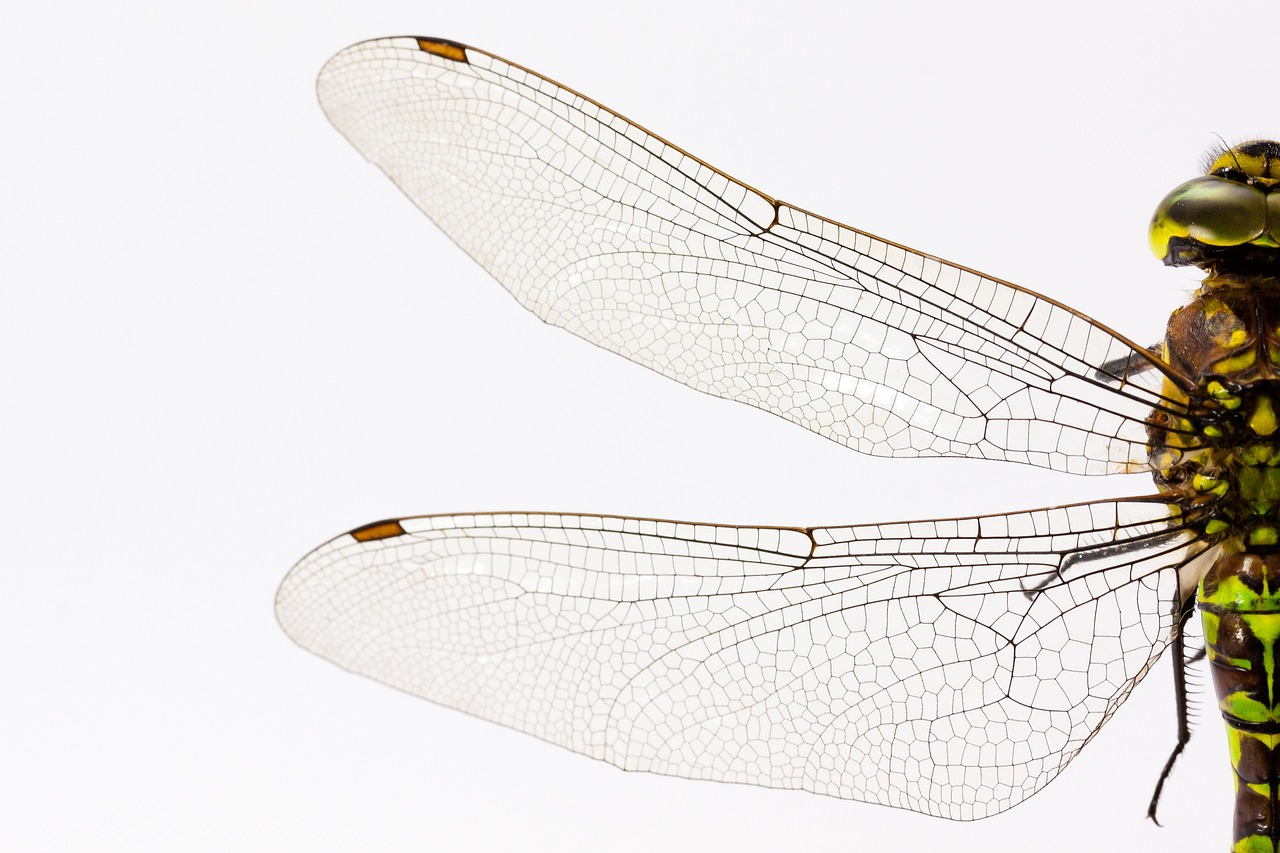
\includegraphics[width=0.45\textwidth]{Images/dragonfly-gf80b992d6_1280.jpg}
    \caption[Dragonfly wings.]{Dragonfly wings are a functional structure constrained by weight.}
    \label{fig:dragonfly}
\end{figure}
Moreover, during the evolutionary process of species, nature has been able to create nano, micro, and macro-structures that provide unique structural properties, adapting shape to function and using only what is truly necessary to achieve the evolutionary goal. Indeed, one of life's principles explained in \citeauthor{baumeister_biomimicry_2011} states \textit{"Life integrates and optimizes these strategies to create conditions conducive to life"}. Therefore, it not only concerns the possibility of creating new multi~-~functional structures with completely new characteristics, but also of doing so by optimizing materials and reducing waste. People have always been fascinated by cellular materials, which is evident from the fact that the first reference to the idea that structure could influence the functional characteristics and behavior of a material was made by Robert Hooke in 1665 \cite{l_gibson_cellular_2010}. Only in recent years, thanks to the computational power of new CAD softwares, it has been possible to experiment with the mechanical characteristics of 3D printed lattice structures. Cellular materials are used mainly for their mechanical characteristics.

\begin{figure}[H]
    \centering
    \subfloat[\label{fig:beehive}]{
        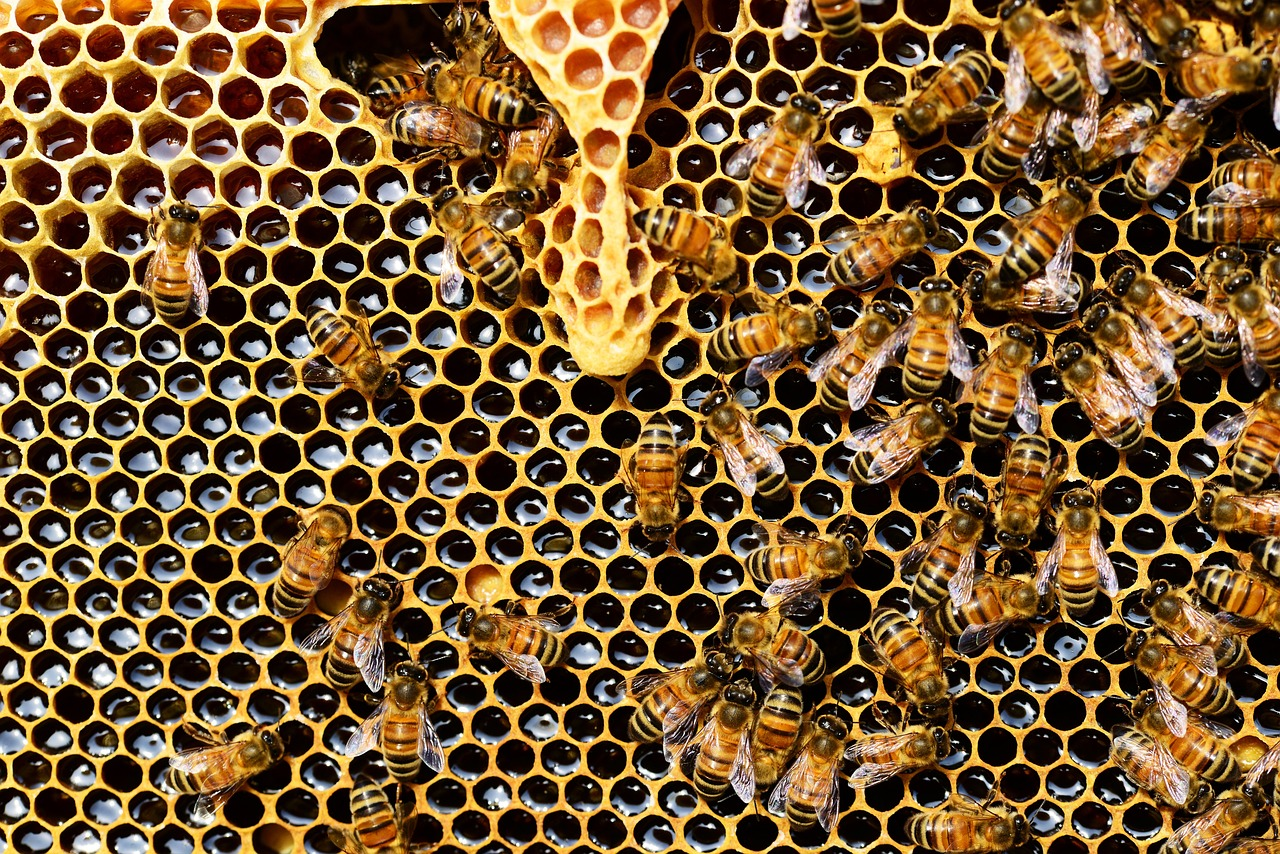
\includegraphics[scale=0.15]{Images/honey-bees-337695_1280.jpg}
    }
    \quad
    \subfloat[\label{fig:beelattice}]{
        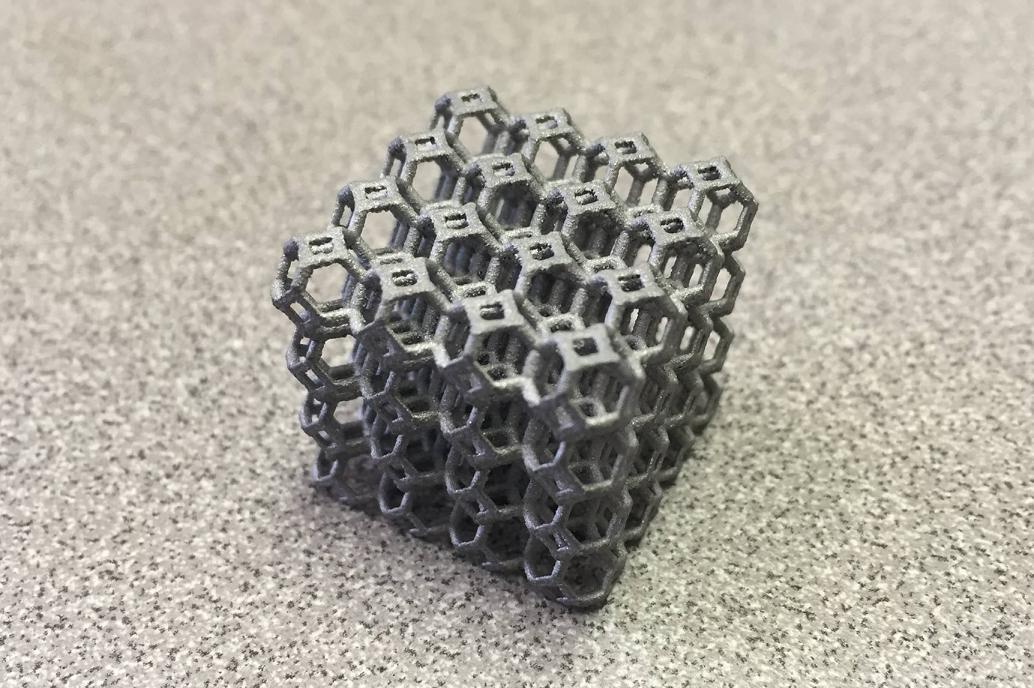
\includegraphics[scale=0.186]{Images/lattice1b.jpg}
    }
    \caption[Bio-inspiration design.]{An example of bio-inspiration design, on the left a beehive and on the right a lattice structure.}
    \label{fig:bioinsp}
\end{figure}

Just think that the aluminum cube in fig. \ref{fig:beelattice} was printed using only \SI{3.9}{g} of material and is able to support a weight of \SI{408}{Kg}, which means it can withstand a stress 100,000 times its weight \cite{noauthor_3d_2014}. If we want to provide a more rigorous framework for classifying the applications of lattice structures in engineering, we can refer to the one proposed by \citeauthor{mcnulty_framework_2017}. According to this framework, cellular structures in nature exist primarily for three reasons:
\begin{itemize}
    \item \textbf{3D space-filling structures}, maybe this is the reason that most closely links the use of cellular structures in nature with AM, namely the need to confer strength to the structure while limiting its weight. Examples of this are the beehive, whose structure provides it with High specific stiffness under self-weight, or toucan's beak in fig. \ref{fig:tucanostruct}, which is characterized by an high bending stiffness;
    \item \textbf{Surface structures}, are structure which enable surfaces to gain specific functional characteristics. For example, veining on the underside of the Amazon water lily leaf in fig. \ref{fig:leafstruct} allows the leaf to gain excellent mechanical resistance, while pomelo skin in fig. \ref{fig:pomelostruct}, with its open-cell structure, enables the fruit to resist impacts;
    \item \textbf{Cylindrical structures}: there are also examples of the use of cellular materials to confer particular characteristics to cylindrical structures (often hollow structure) that would otherwise be too fragile. For example in fig. \ref{fig:hedgehogstruct} there is a hedgehog quill and the particular structure confers ovalization and buckling resistance to the structure and in fig. \ref{fig:bananostruct} there is the section of the petiole of a banana, which is characterized by an high bending stiffness but also a torsional flexibility.
\end{itemize}
\begin{figure}[H]
    \centering
    \subfloat[Toucan beak section.\label{fig:tucanostruct}]{
        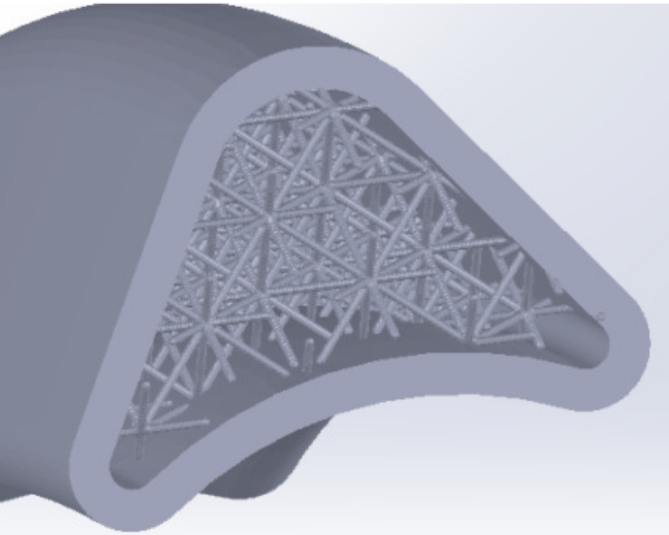
\includegraphics[scale=0.4]{Images/tucano.png}
    }
    \qquad
    \subfloat[Amazon Waterlily leaf underside.\label{fig:leafstruct}]{
        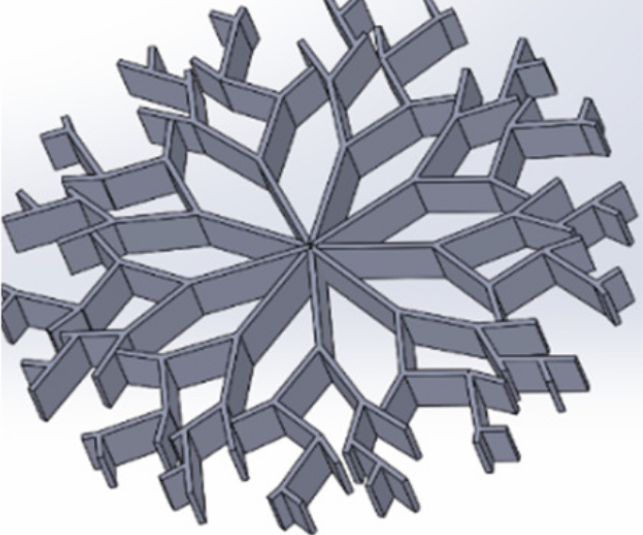
\includegraphics[scale=0.4]{Images/leaf.png}
    }
    \qquad
     \subfloat[Pomelo skin section.\label{fig:pomelostruct}]{
        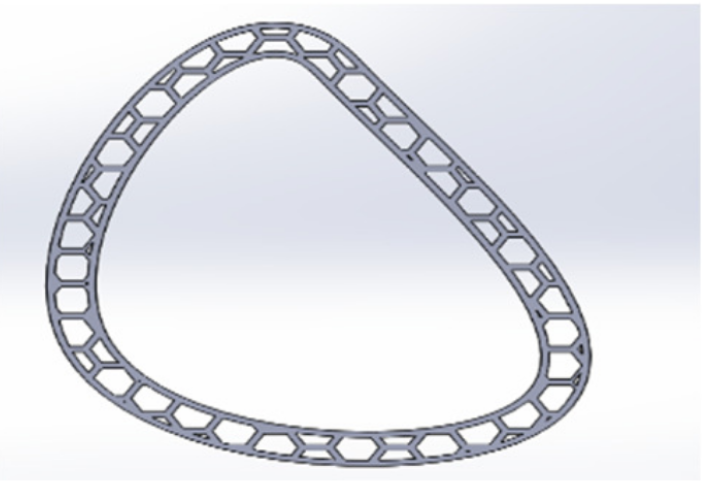
\includegraphics[scale=0.4]{Images/pomelo.png}
    }
    \qquad
    \subfloat[Hedgehog quill section.\label{fig:hedgehogstruct}]{
        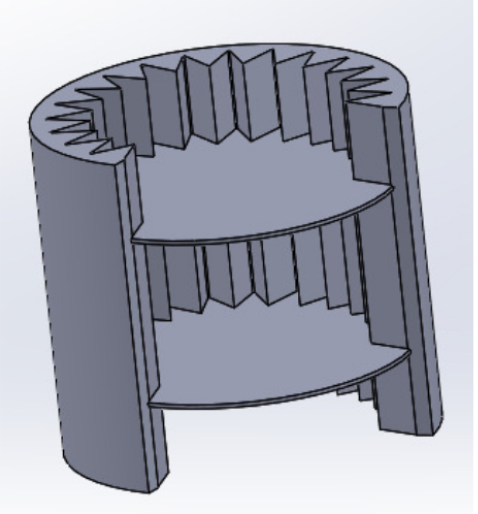
\includegraphics[scale=0.4]{Images/edgehog.png}
    }
    \qquad
    \subfloat[Section of a banana petiole.\label{fig:bananostruct}]{
        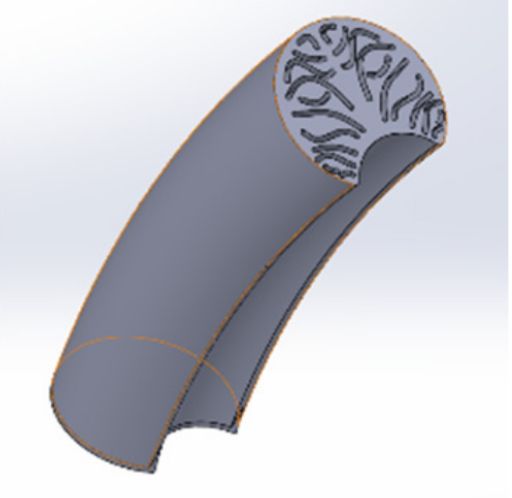
\includegraphics[scale=0.4]{Images/banano.png}
    }
    \caption[Cellular materials in nature]{Some examples of cellular materials in nature. Adapted from \citeauthor{mcnulty_framework_2017} (\citeyear{mcnulty_framework_2017}).}
    \label{fig:cellstruct}
\end{figure}
Lattice structures are versatile and can be effectively applied in various engineering fields to address multiple challenges. Specifically, they are commonly used in four main areas \cite{bhate_classification_2019}: structural engineering for vibration control, strain isolation, and weight reduction purposes; thermal engineering for applications such as heat exchangers, flame arresters, or heat shields; fluid dynamics engineering, where lattice structures can serve as catalyst carriers or packaging; and in biological engineering, where they can be leveraged for bone integration in prosthetic and cell growth. Due to their unique properties, lattice structures are an attractive choice for engineers and designers seeking innovative solutions to complex problems across a wide range of industries, especially in the automotive, aerospace, energy and commodities, and medical industries.
\subsection{Successful Case Studies for Lattice Structures} \label{subsec:casestudieslattice}
In this section, we will discuss some relevant case studies of successful applications of lattice structures. We will not focus on a single industry but rather analyze applications in various fields.
\section{Defects in 3d-printed metal objects}
\subsection{Classical indicators for lattice structures quality}
% ---------






In this chapter additional useful information are reported.

\section{Sections and subsections}
\label{sec:section_name}
Chapters are typically subdivided into sections and subsections, and, optionally,
subsubsections, paragraphs and subparagraphs.
All can have a title, but only sections and subsections are numbered.
A new section is created by the command
\begin{verbatim}
\section{Title of the section}
\end{verbatim}
The numbering can be turned off by using \verb|\section*{}|.
\\
A new subsection is created by the command
\begin{verbatim}
\subsection{Title of the subsection}
\end{verbatim}
and, similarly, the numbering can be turned off by adding an asterisk as follows 
\begin{verbatim}
\subsection*{}
\end{verbatim}

\section{Equations}
\label{sec:eqs}
This section gives some examples of writing mathematical equations in your thesis.

Maxwell's equations read:
\begin{subequations}
    \label{eq:maxwell}
    \begin{align}[left=\empheqlbrace]
    \nabla\cdot \bm{D} & = \rho, \label{eq:maxwell1} \\
    \nabla \times \bm{E} +  \frac{\partial \bm{B}}{\partial t} & = \bm{0}, \label{eq:maxwell2} \\
    \nabla\cdot \bm{B} & = 0, \label{eq:maxwell3} \\
    \nabla \times \bm{H} - \frac{\partial \bm{D}}{\partial t} &= \bm{J}. \label{eq:maxwell4}
    \end{align}
\end{subequations}

Equation~\eqref{eq:maxwell} is automatically labeled by \texttt{cleveref},
as well as Equation~\eqref{eq:maxwell1} and Equation~\eqref{eq:maxwell3}.
Thanks to the \verb|cleveref| package, there is no need to use \verb|\eqref|.
Remember that Equations have to be numbered only if they are referenced in the text.

Equations~\eqref{eq:maxwell_multilabels1}, \eqref{eq:maxwell_multilabels2}, \eqref{eq:maxwell_multilabels3}, and \eqref{eq:maxwell_multilabels4} show again Maxwell's equations without brace:
\begin{align}
    \nabla\cdot \bm{D} & = \rho, \label{eq:maxwell_multilabels1} \\
    \nabla \times \bm{E} +  \frac{\partial \bm{B}}{\partial t} &= \bm{0}, \label{eq:maxwell_multilabels2} \\
    \nabla\cdot \bm{B} & = 0, \label{eq:maxwell_multilabels3} \\
    \nabla \times \bm{H} - \frac{\partial \bm{D}}{\partial t} &= \bm{J} \label{eq:maxwell_multilabels4}.
\end{align}

Equation~\eqref{eq:maxwell_singlelabel} is the same as before,
but with just one label:
\begin{equation}
    \label{eq:maxwell_singlelabel}
    \left\{
    \begin{aligned}
    \nabla\cdot \bm{D} & = \rho, \\
    \nabla \times \bm{E} +  \frac{\partial \bm{B}}{\partial t} &= \bm{0},\\
    \nabla\cdot \bm{B} & = 0, \\
    \nabla \times \bm{H} - \frac{\partial \bm{D}}{\partial t} &= \bm{J}.
    \end{aligned}
    \right.
\end{equation}

\section{Figures, Tables and Algorithms}
Figures, Tables and Algorithms have to contain a Caption that describe their content, and have to be properly reffered in the text.

\subsection{Figures}
\label{subsec:figures}

For including pictures in your text you can use \texttt{TikZ} for high-quality hand-made figures,
or just include them as usual with the command
\begin{verbatim}
\includegraphics[options]{filename.xxx}
\end{verbatim}
Here xxx is the correct format, e.g. \verb|.png|, \verb|.jpg|, \verb|.eps|, \dots.

\begin{figure}[H]
    \centering
    
\includegraphics[width=0.3\textwidth]{logo_polimi_scritta.eps}
    \caption{Caption of the Figure to appear in the List of Figures.}
    \label{fig:quadtree}
\end{figure}

Thanks to the \texttt{\textbackslash subfloat} command, a single figure, such as Figure~\ref{fig:quadtree},
can contain multiple sub-figures with their own caption and label, e.g. \color{black} Figure~\ref{fig:polimi_logo1} and Figure~\ref{fig:polimi_logo2}. 

\begin{figure}[H]
    \centering
    \subfloat[One PoliMi logo.\label{fig:polimi_logo1}]{
        
\includegraphics[scale=0.5]{Images/logo_polimi_scritta.eps}
    }
    \quad
    \subfloat[Another one PoliMi logo.\label{fig:polimi_logo2}]{
        
\includegraphics[scale=0.5]{Images/logo_polimi_scritta2.eps}
    }
    \caption[Shorter caption]{This is a very long caption you don't want to appear in the List of Figures.}
    \label{fig:quadtree2}
\end{figure}


\subsection{Tables}
\label{subsec:tables}

Within the environments \texttt{table} and  \texttt{tabular} you can create very fancy tables as the one shown in Table~\ref{table:example}.
\begin{table}[H]
    \caption*{\textbf{Title of Table (optional)}}
    \centering 
    \begin{tabular}{|p{3em} c c c |}
    \hline
    \rowcolor{bluepoli!40} % comment this line to remove the color
     & \textbf{column 1} & \textbf{column 2} & \textbf{column 3} \T\B \\
    \hline \hline
    \textbf{row 1} & 1 & 2 & 3 \T\B \\
    \textbf{row 2} & $\alpha$ & $\beta$ & $\gamma$ \T\B\\
    \textbf{row 3} & alpha & beta & gamma \B\\
    \hline
    \end{tabular}
    \\[10pt]
    \caption{Caption of the Table to appear in the List of Tables.}
    \label{table:example}
\end{table}


\subsection{Algorithms}
\label{subsec:algorithms}

Pseudo-algorithms can be written in \LaTeX{} with the \texttt{algorithm} and \texttt{algorithmic} packages.
An example is shown in Algorithm~\ref{alg:var}.
\begin{algorithm}[H]
    \label{alg:example}
    \caption{Name of the Algorithm}
    \label{alg:var}
    \label{protocol1}
    \begin{algorithmic}[1]
    \STATE Initial instructions
    \FOR{$for-condition$}
    \STATE{Some instructions}
    \IF{$if-condition$}
    \STATE{Some other instructions}
    \ENDIF
    \ENDFOR
    \WHILE{$while-condition$}
    \STATE{Some further instructions}
    \ENDWHILE
    \STATE Final instructions
    \end{algorithmic}
\end{algorithm} 

\vspace{5mm}

\section{Theorems, propositions and lists}

\subsection{Theorems}
Theorems have to be formatted as:
\begin{theorem}
\label{a_theorem}
Write here your theorem. 
\end{theorem}
\textit{Proof.} If useful you can report here the proof.

\subsection{Propositions}
Propositions have to be formatted as:
\begin{proposition}
Write here your proposition.
\end{proposition}

\subsection{Lists}
How to  insert itemized lists:
\begin{itemize}
    \item first item;
    \item second item.
\end{itemize}
How to insert numbered lists:
\begin{enumerate}
    \item first item;
    \item second item.
\end{enumerate}

\section{Use of copyrighted material}

Each student is responsible for obtaining copyright permissions, if necessary, to include published material in the thesis.
This applies typically to third-party material published by someone else.

\section{Plagiarism}

You have to be sure to respect the rules on Copyright and avoid an involuntary plagiarism.
It is allowed to take other persons' ideas only if the author and his original work are clearly mentioned.
As stated in the Code of Ethics and Conduct, Politecnico di Milano \textit{promotes the integrity of research,
condemns manipulation and the infringement of intellectual property}, and gives opportunity to all those
who carry out research activities to have an adequate training on ethical conduct and integrity while doing research.
To be sure to respect the copyright rules, read the guides on Copyright legislation and citation styles available
at:
\begin{verbatim}
https://www.biblio.polimi.it/en/tools/courses-and-tutorials
\end{verbatim}
You can also attend the courses which are periodically organized on "Bibliographic citations and bibliography management".

\section{Bibliography and citations}
Your thesis must contain a suitable Bibliography which lists all the sources consulted on developing the work.
The list of references is placed at the end of the manuscript after the chapter containing the conclusions.
We suggest to use the BibTeX package and save the bibliographic references  in the file \verb|Thesis_bibliography.bib|.
This is indeed a database containing all the information about the references. To cite in your manuscript, use the \verb|\cite{}| command as follows:
\\
\textit{Here is how you cite bibliography entries:  or multiple ones at once}.
\\
The bibliography and list of references are generated automatically by running BibTeX .

\chapter{Conclusions and future developments}
\label{ch:conclusions}%
A final chapter containing the main conclusions of your research/study
and possible future developments of your work have to be inserted in this chapter.

%-------------------------------------------------------------------------
%	BIBLIOGRAPHY
%-------------------------------------------------------------------------

\addtocontents{toc}{\vspace{2em}} % Add a gap in the Contents, for aesthetics
\bibliography{references}

%-------------------------------------------------------------------------
%	APPENDICES
%-------------------------------------------------------------------------

\cleardoublepage
\addtocontents{toc}{\vspace{2em}} % Add a gap in the Contents, for aesthetics
\appendix
\chapter{Appendix A}
If you need to include an appendix to support the research in your thesis, you can place it at the end of the manuscript.
An appendix contains supplementary material (figures, tables, data, codes, mathematical proofs, surveys, \dots)
which supplement the main results contained in the previous chapters.

\chapter{Appendix B}
It may be necessary to include another appendix to better organize the presentation of supplementary material.


% LIST OF FIGURES
\listoffigures

% LIST OF TABLES
\listoftables

% LIST OF SYMBOLS
% Write out the List of Symbols in this page
\chapter*{List of Symbols} % You have to include a chapter for your list of symbols (
\begin{table}[H]
    \centering
    \begin{tabular}{lll}
        \textbf{Variable} & \textbf{Description} & \textbf{SI unit} \\\hline\\[-9px]
        $\bm{u}$ & solid displacement & m \\[2px]
        $\bm{u}_f$ & fluid displacement & m \\[2px]
    \end{tabular}
\end{table}

% ACKNOWLEDGEMENTS
\chapter*{Acknowledgements}
Here you might want to acknowledge someone.

\cleardoublepage

\end{document}
